\documentclass[11pt,a4paper]{article}
\usepackage[utf8]{inputenc}
\usepackage[T1]{fontenc}
\usepackage[spanish]{babel}
\usepackage[a4paper,margin=2.2cm]{geometry}
\usepackage{graphicx}
\usepackage{booktabs}
\usepackage{amsmath}
\usepackage{float}
\usepackage[hidelinks]{hyperref}
\usepackage{caption}
\usepackage{array}

\graphicspath{{figures/}}
\setlength{\parindent}{0pt}
\setlength{\parskip}{0.55em}

\title{Segmentación de miotubos en imágenes de microscopía\\
\large Informe de EDA, partición de datos y resultados experimentales}
\author{Proyecto myotubes-seg}
\date{20 de noviembre de 2026}

\begin{document}
\maketitle
\tableofcontents
\newpage

\section{Objetivo y alcance}

El objetivo fue preparar el conjunto de datos \texttt{vt} y comparar métodos para segmentar miotubos en imágenes de microscopía. El análisis cubre el inventario disponible, la calidad de las anotaciones, el riesgo de fuga entre particiones y la evaluación de dos líneas base clásicas. También se describen dos entrenamientos YOLOv11-seg realizados sobre el conjunto preparado.

La evaluación final de las líneas base se realizó sobre validación. El conjunto de prueba permanece reservado para una evaluación independiente posterior.

\section{Datos y análisis exploratorio}

El inventario contiene 306 imágenes. La resolución original es aproximadamente 2592 por 1944 píxeles. La medida de área cubierta por miotubos es muy baja: el 1.759\% del área total de las máscaras corresponde a miotubo. Las máscaras contienen 2.148 instancias. En el conjunto original, 34 imágenes están vacías y aparecen como instancias sin anotar.

\begin{figure}[H]
\centering
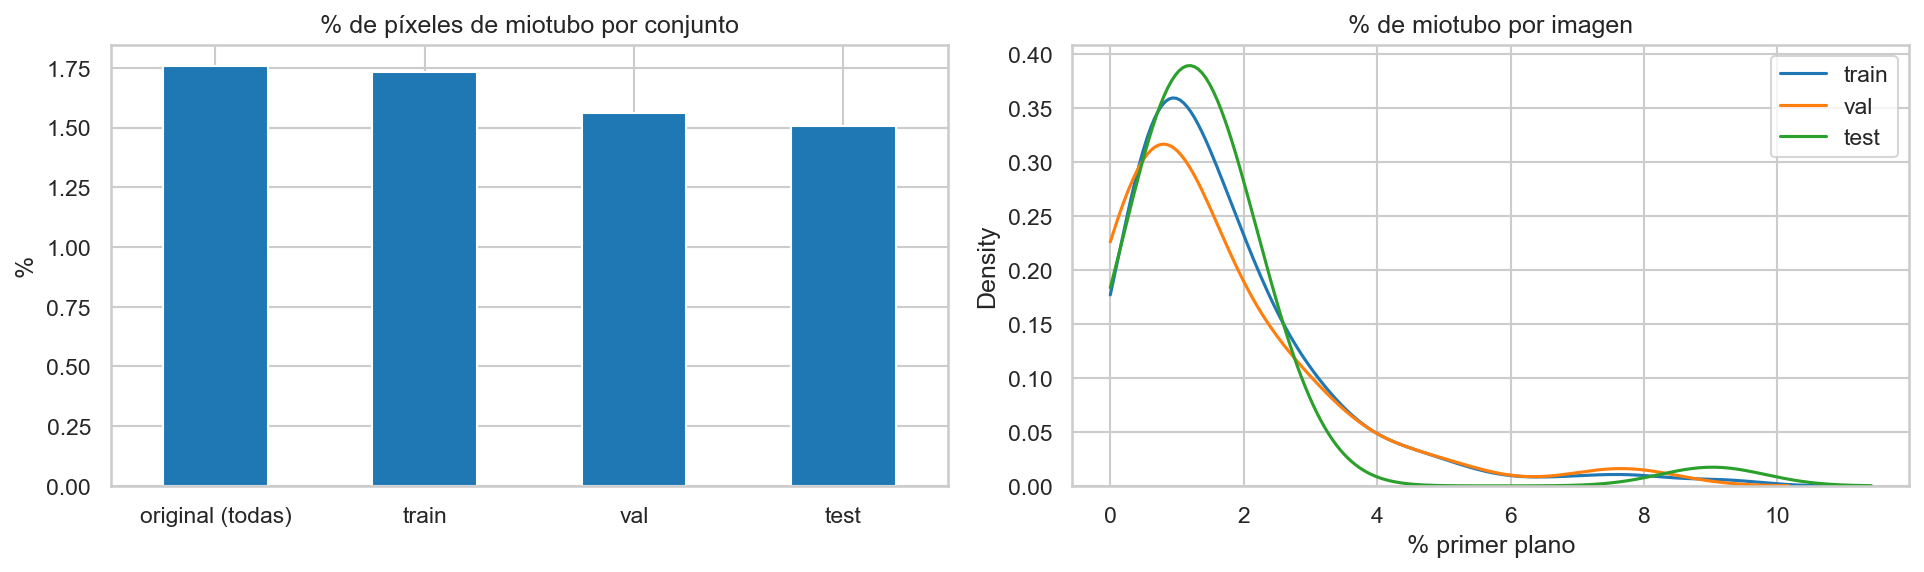
\includegraphics[width=0.78\textwidth]{fig_desbalance.png}
\caption{Desbalance entre miotubo y fondo en los conjuntos disponibles.}
\label{fig:desbalance}
\end{figure}

La mediana del área anotada por imagen es 0.861\%, aunque existen imágenes con áreas mucho mayores. Esta variabilidad produce diferencias importantes entre ejemplos. Las mascaras vacías no deben interpretarse como negativos confirmados, pues algunas contienen miotubos visibles sin anotación.

\subsection{Calidad de las etiquetas}

Las etiquetas YOLO y las máscaras PNG representan la misma geometría con elevada coherencia global: la mediana del IoU entre la rasterización YOLO y la máscara PNG es 0.9583, con media 0.9576. Sin embargo, 51 imágenes tienen un IoU inferior a 0.95. Las diferencias pueden deberse a conversiones de contorno, resolución o errores puntuales en la anotación.

Las mascaras usan 34 imágenes sin instancias y se excluyen del entrenamiento y la validación como anotaciones vacías o no confiables. También se excluyen imágenes con una caja mayor al 20\% del área.

\begin{figure}[H]
\centering
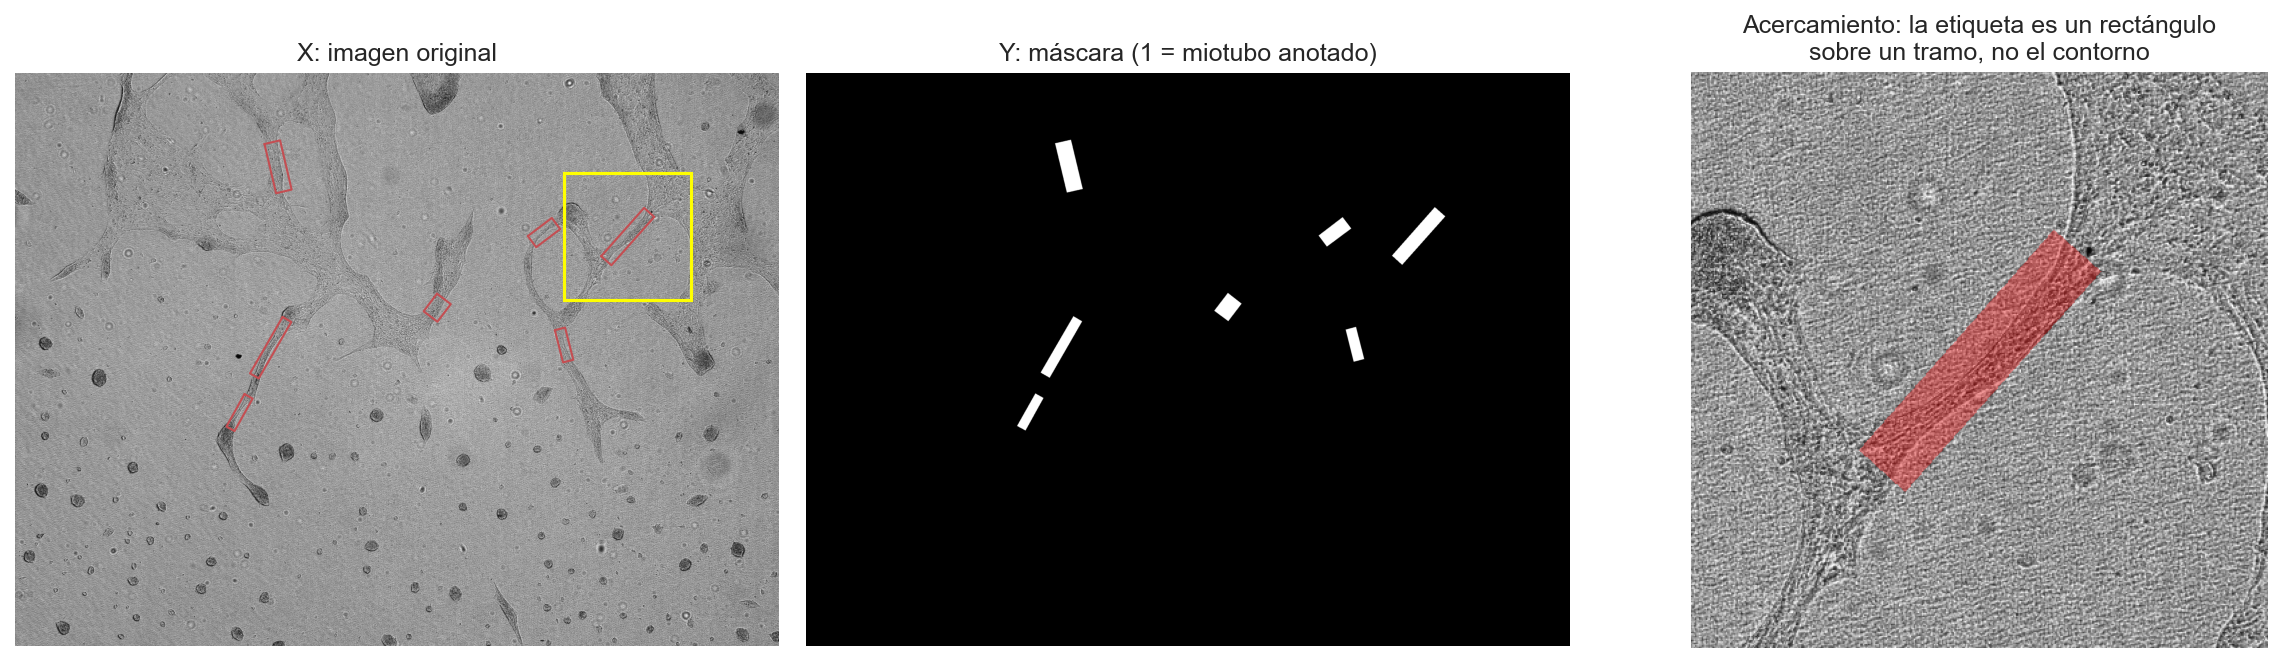
\includegraphics[width=0.76\textwidth]{fig_etiqueta.png}
\caption{Ejemplos de imagen, máscara y etiqueta utilizados en el análisis exploratorio.}
\label{fig:etiqueta}
\end{figure}

\subsection{Duplicados y riesgo de fuga}

Las imágenes presentan una estructura de réplicas que no puede ignorarse. Se encontraron 117 pares casi duplicados con distancia dHash menor o igual a 6, incluidos 16 pares idénticos. Hay 54 clústeres con al menos dos copias y 138 imágenes involucradas en copias. Además, 109 pares presentan una anotación distinta con IoU inferior a 0.9.

Una partición aleatoria puede colocar réplicas en entrenamiento y validación. En 50 semillas, el promedio de imágenes de validación con copia en entrenamiento fue 36.2\%, con un máximo de 56.5\%. Por este motivo no se utilizó una partición aleatoria simple.

\begin{figure}[H]
\centering
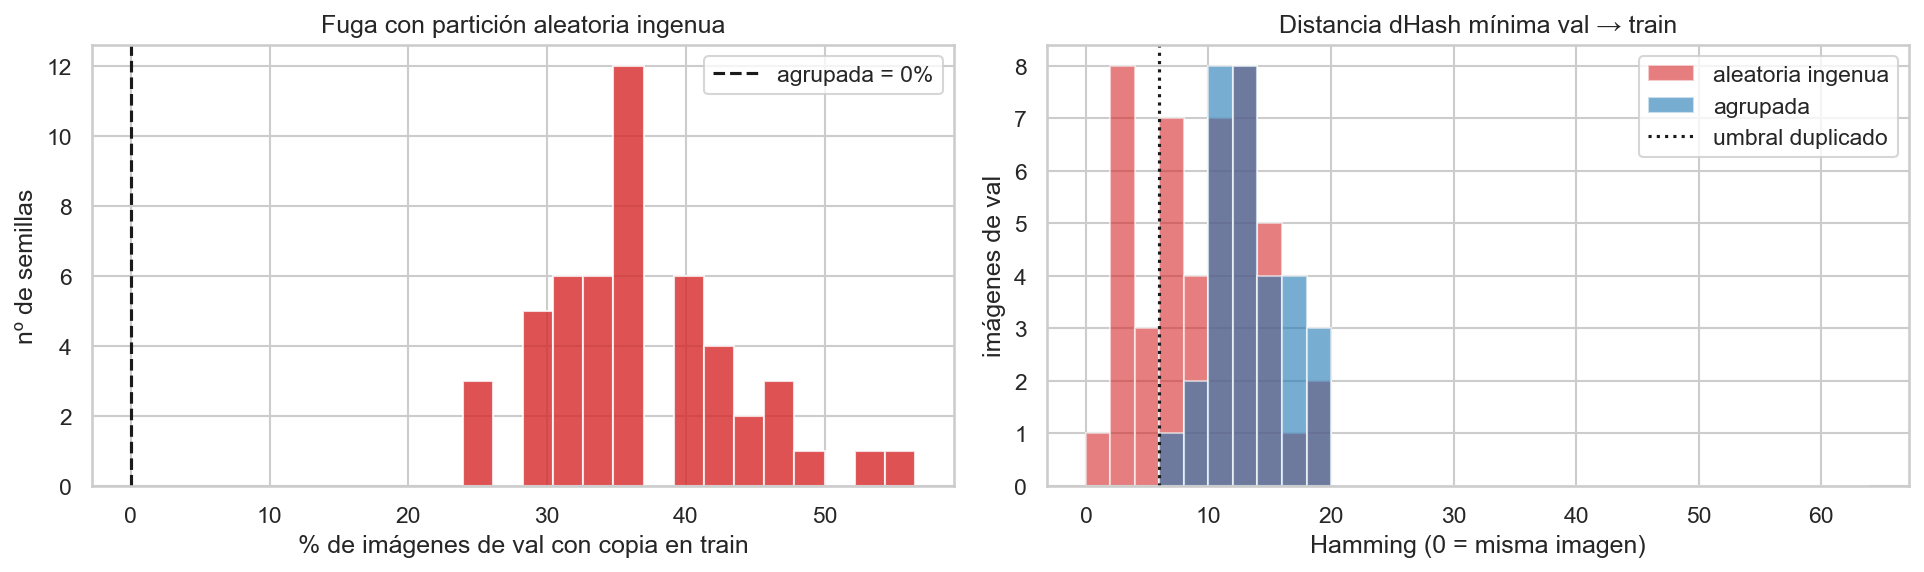
\includegraphics[width=0.78\textwidth]{fig_fuga.png}
\caption{Comparación entre partición aleatoria ingenua y partición agrupada.}
\label{fig:fuga}
\end{figure}

La partición final agrupa por duplicados y por identificador de célula. El mismo método evita toda coincidencia de validación con entrenamiento bajo el criterio utilizado. También se detectó que agrupar por UUID puede concentrar el 44\% de las imágenes en un solo grupo, por lo que esa opción no se utilizó.

\section{Preparación de los datos}

La selección excluye máscaras vacías y imágenes con una instancia desproporcionadamente grande. Los duplicados se deduplican conservando una copia por clúster, preferentemente la imagen con mayor área anotada. Los grupos completos se asignaron a entrenamiento, validación y prueba con proporciones 70/15/15 y semilla 42.

\begin{table}[H]
\centering
\caption{Tamaño y desbalance de las particiones.}
\begin{tabular}{lrrrrr}
\toprule & \multicolumn{1}{c}{Imágenes} & \multicolumn{1}{c}{Instancias} & \multicolumn{1}{c}{Miotubo} & \multicolumn{1}{c}{Fondo/miotubo} & \multicolumn{1}{c}{Imágenes vacías}\\
\midrule
Original & 306 & 2148 & 1.759\% & 55.84 & 34\\
Entrenamiento & 136 & 1144 & 1.734\% & 56.68 & 0\\
Validación & 30 & 218 & 1.563\% & 62.99 & 0\\
Prueba & 29 & 327 & 1.505\% & 65.45 & 0\\
\bottomrule
\end{tabular}
\label{tab:particion}
\end{table}

Después de las exclusiones y la deduplicación, quedan 136 imágenes de entrenamiento, 30 de validación y 29 de prueba. Las 74 imágenes descartadas por duplicado y las 37 excluidas se mantienen registradas sin eliminar los originales.

\section{Líneas base}

Se compararon dos métodos sin aprendizaje profundo sobre validación a escala 0.25. La escala reduce las imágenes a 648 por 486. El umbral de clasificación se ajustó únicamente con entrenamiento.

\subsection{Método clásico}

La primera línea base combina filtro de Sato, umbral y operaciones morfológicas. El método obtuvo 0.7202 de ROC-AUC y 0.0666 de PR-AUC, frente a una prevalencia aleatoria de 0.0156.

A nivel píxel, el IoU del miotubo fue 0.0831 y el Dice fue 0.1535. La precisión fue 0.1008 y el recall 0.3222. No se encontró ningún umbral que alcanzara precisión global de al menos 0.80.

\subsection{Clasificador de píxeles}

La segunda línea base utiliza características locales y HistGradientBoosting. El modelo alcanzó 0.8968 de ROC-AUC y 0.1763 de PR-AUC. El umbral seleccionado en entrenamiento fue 0.8890 y se evaluó con 0.9822 en validación.

El IoU del miotubo fue 0.1650 y el Dice 0.2832. La precisión fue 0.3084 y el recall 0.2618. El recall con precisión de al menos 0.80 fue 0.0003.

\begin{table}[H]
\centering
\caption{Resultados de las líneas base en validación.}
\begin{tabular}{lrrrrrr}
\toprule
Método & PR-AUC & ROC-AUC & IoU & Dice & Precisión & Recall\\
\midrule
Clásica & 0.0666 & 0.7202 & 0.0831 & 0.1535 & 0.1008 & 0.3222\\
Caracteristicas con HGB & 0.1763 & 0.8968 & 0.1650 & 0.2832 & 0.3084 & 0.2618\\
\bottomrule
\end{tabular}
\label{tab:baselines}
\end{table}

La diferencia entre los dos métodos es clara en PR-AUC, ROC-AUC e IoU. El clasificador basado en características supera al filtro clásico. Incluso así, el rendimiento sobre miotubos sigue siendo limitado por el desbalance y la variabilidad de apariencia.

\begin{figure}[H]
\centering
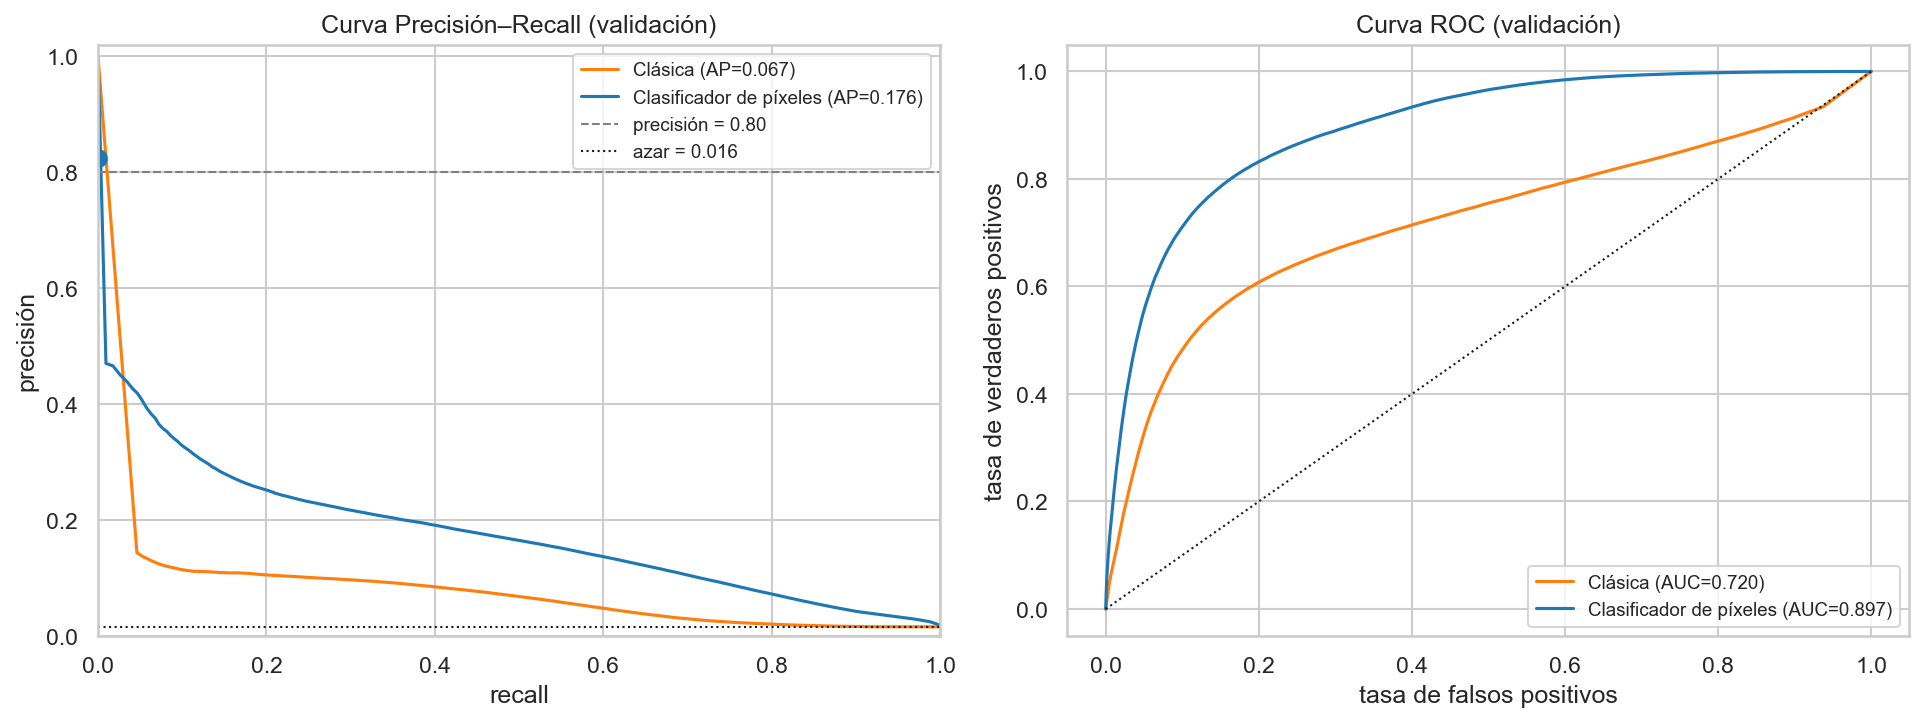
\includegraphics[width=0.78\textwidth]{fig_pr_roc.png}
\caption{Curvas precisión-recall y ROC para las dos líneas base.}
\label{fig:prroc}
\end{figure}

\begin{figure}[H]
\centering
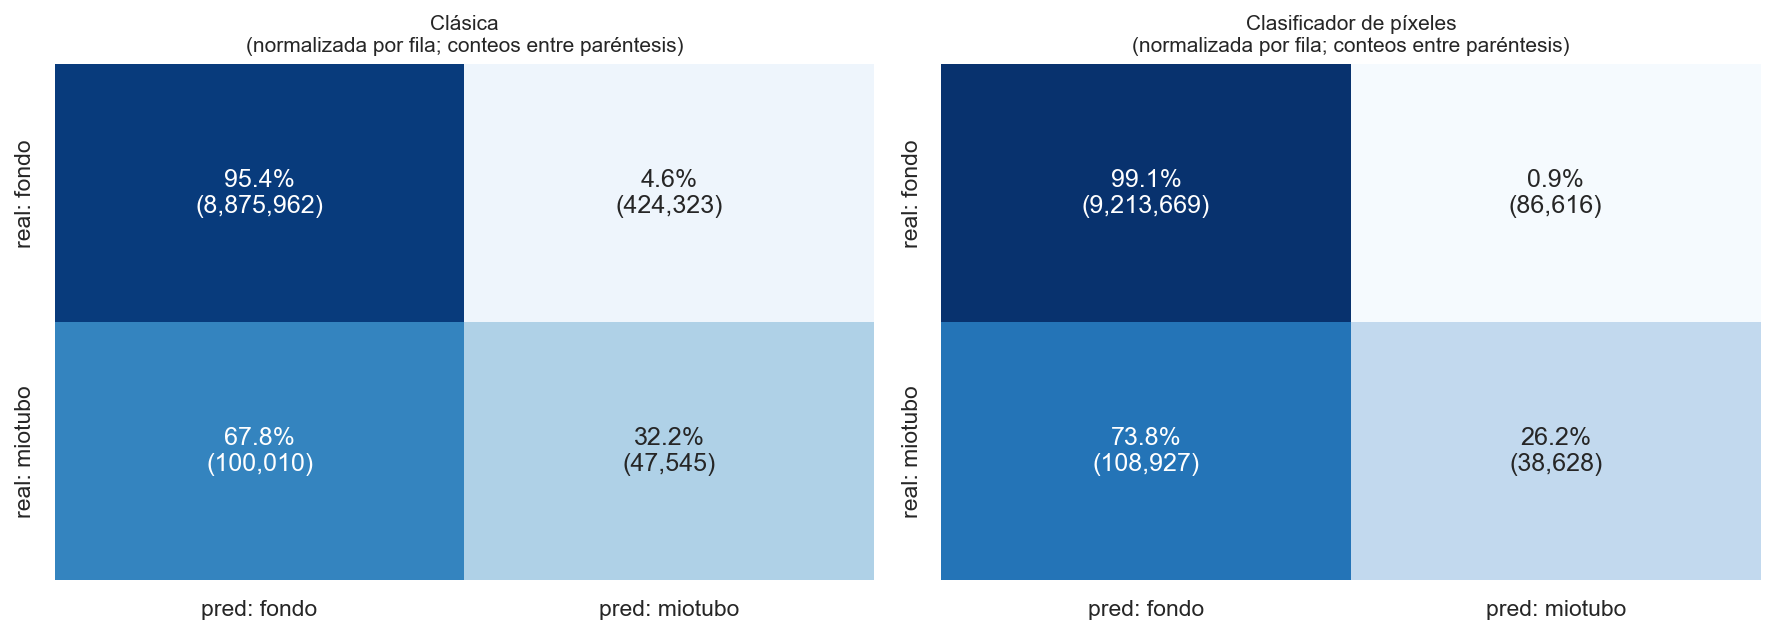
\includegraphics[width=0.78\textwidth]{fig_confusion.png}
\caption{Matrices de confusión de las líneas base.}
\label{fig:confusion}
\end{figure}

\begin{figure}[H]
\centering
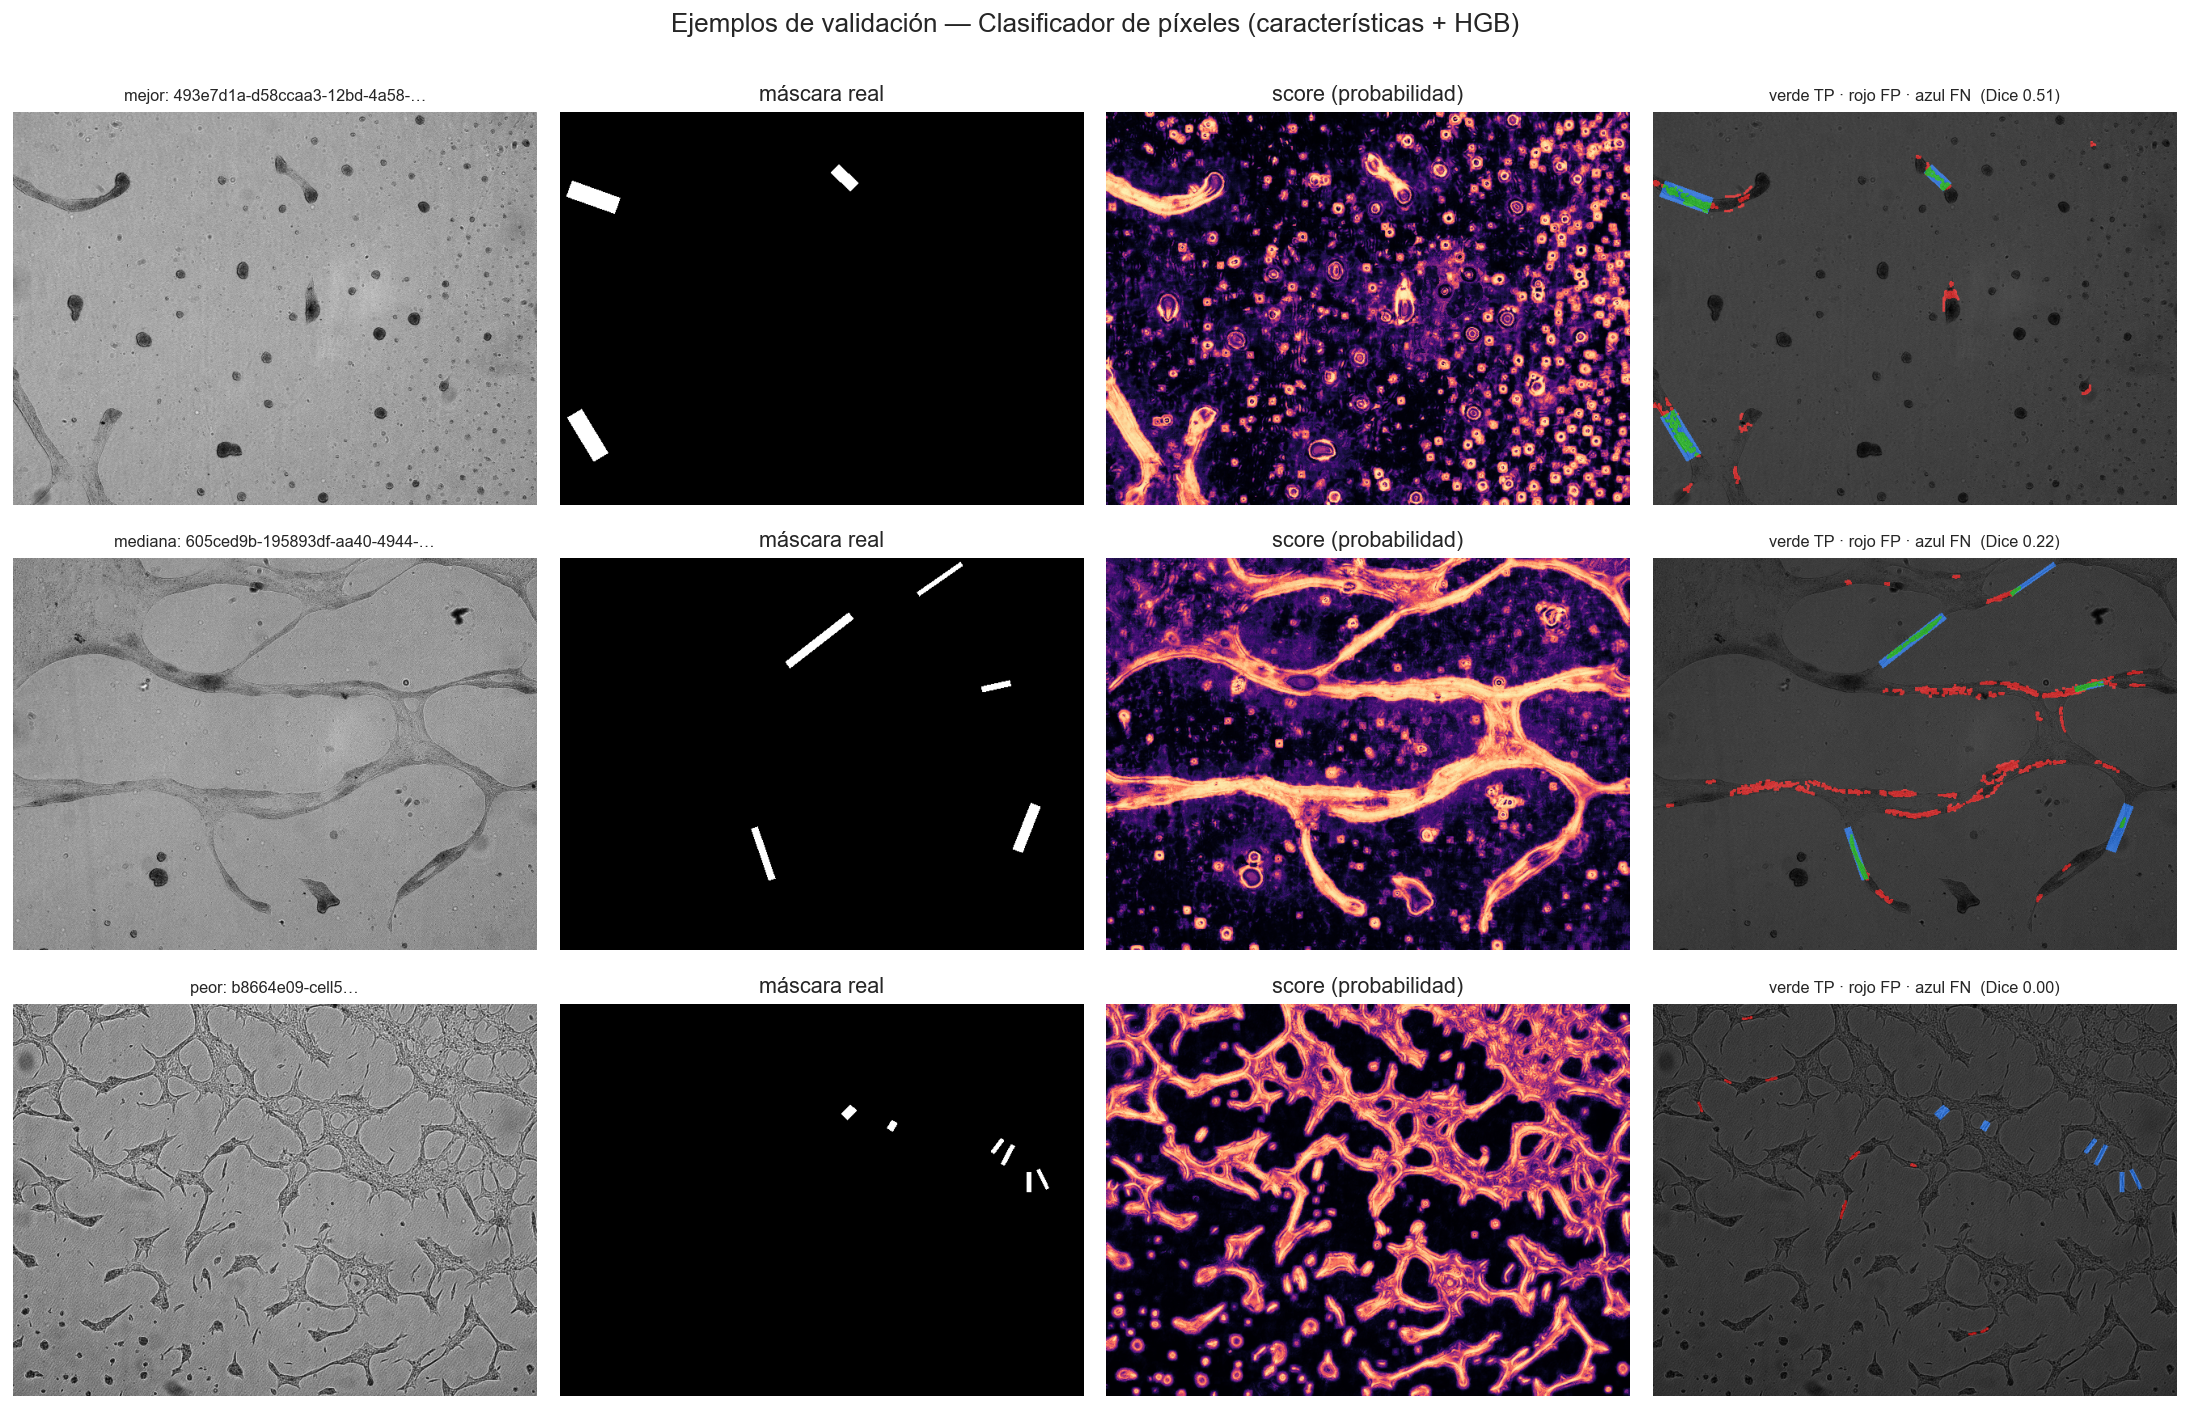
\includegraphics[width=0.82\textwidth]{fig_cualitativo.png}
\caption{Comparación cualitativa de las predicciones sobre ejemplos de validación.}
\label{fig:cualitativo}
\end{figure}

Las curvas por imagen muestran una variabilidad amplia. Para el clasificador de píxeles, algunas imágenes alcanzan Dice aceptable, pero otras quedan cerca de cero. El método clásico presenta dispersión similar y valores menores en general.

\begin{figure}[H]
\centering
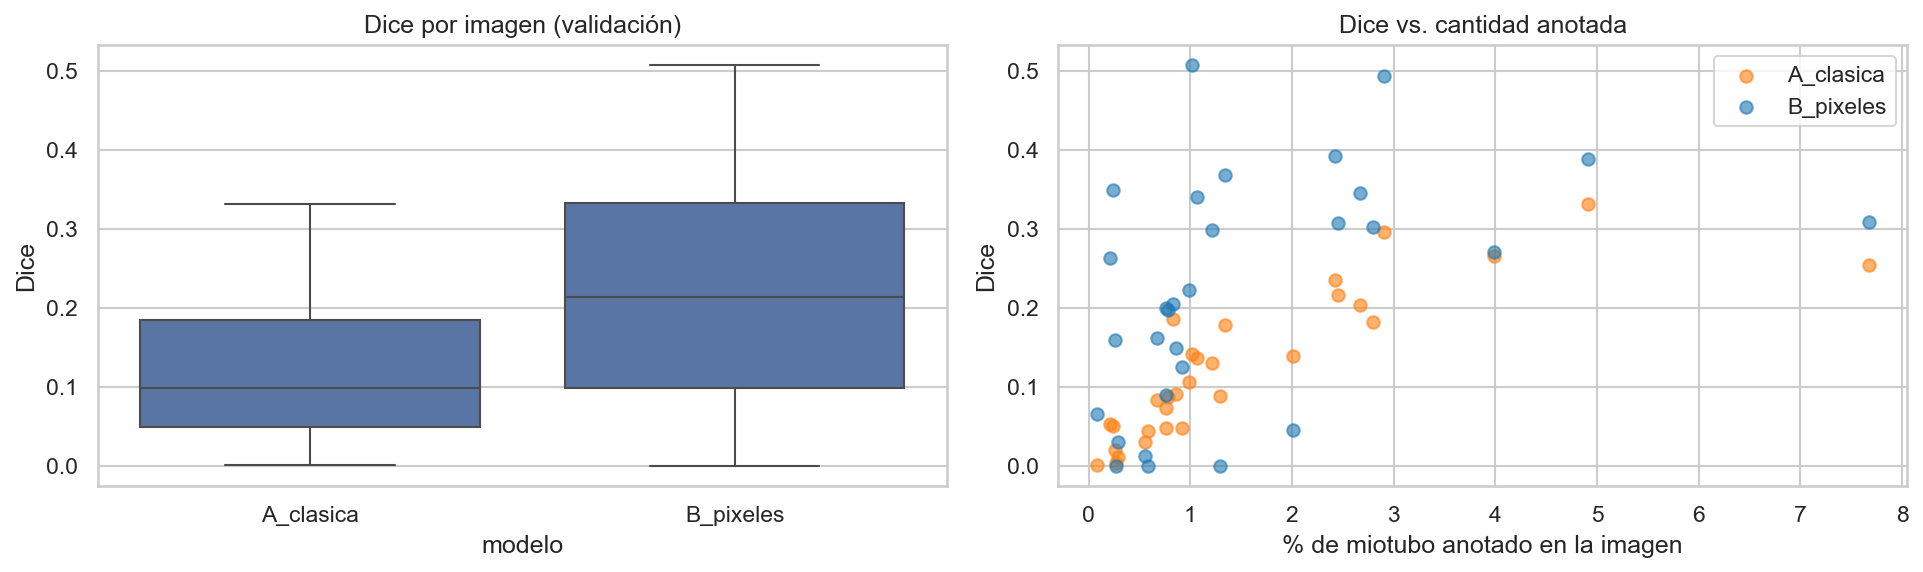
\includegraphics[width=0.78\textwidth]{fig_por_imagen.png}
\caption{Distribución de métricas por imagen en validación.}
\label{fig:porimagen}
\end{figure}

\section{Experimentos YOLOv11-seg}

Se entrenaron dos variantes YOLOv11-seg con una clase, 50 épocas, resolución de 1024 píxeles y semilla 42. La variante de transferencia congeló las primeras 10 capas. La variante fine-tune actualizó todos los parámetros.

Ambos entrenamientos convergieron lentamente y muestran resultados modestos en validación. En el entrenamiento de transferencia, el mayor mAP50 de máscaras fue 0.4364 en la época 50. La precisión de máscaras fue 0.4574 y el recall 0.4690 en esa época. El mayor mAP50-95 fue 0.1596 en la época 33.

En fine-tune, el mayor mAP50 de máscaras fue 0.4763 en la época 48. La precisión fue 0.4891 y el recall 0.5379 en esa época. El mayor mAP50-95 fue 0.1692 en la época 45.

\begin{table}[H]
\centering
\caption{Máximos principales de los entrenamientos YOLOv11-seg.}
\begin{tabular}{lrrrr}
\toprule
Experimento & mAP50 máscara & Época & mAP50-95 máscara & Época\\
\midrule
Transferencia & 0.4364 & 50 & 0.1596 & 33\\
Fine-tune & 0.4763 & 48 & 0.1692 & 45\\
\bottomrule
\end{tabular}
\label{tab:yolo}
\end{table}

\begin{figure}[H]
\centering
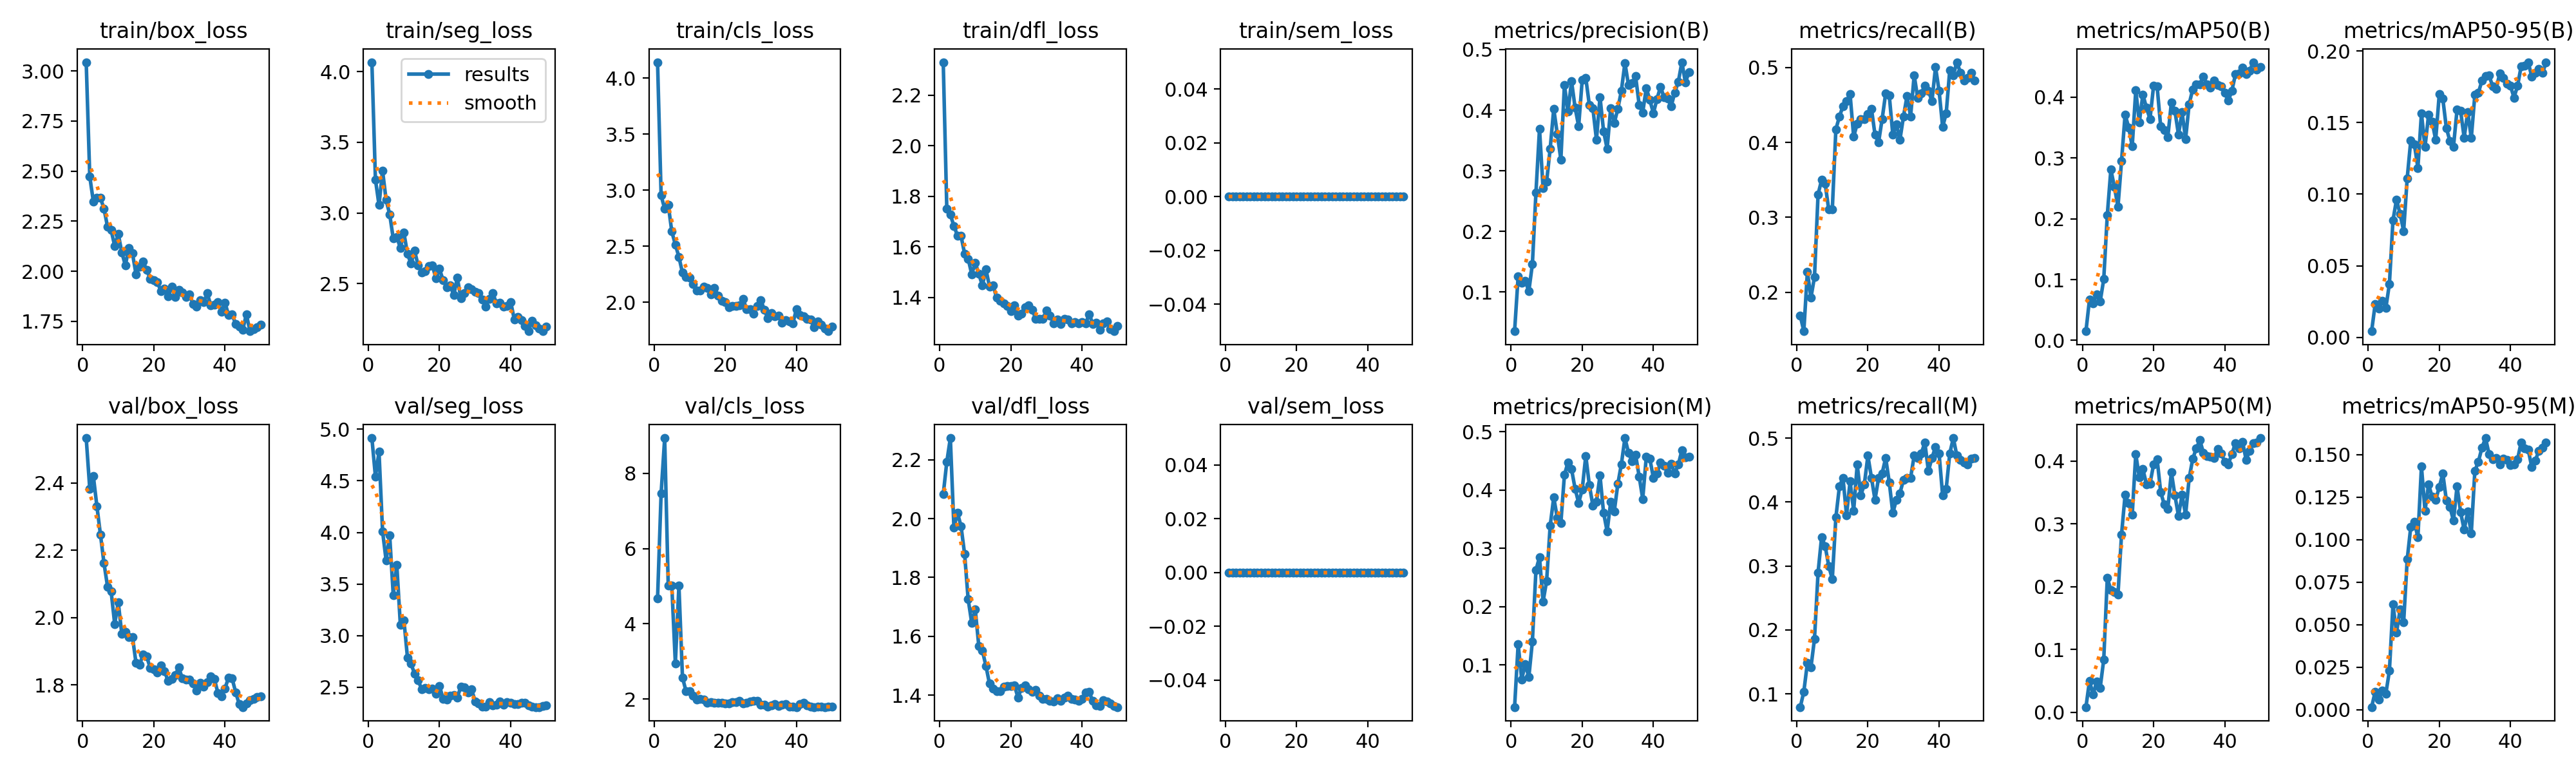
\includegraphics[width=0.86\textwidth]{yolo_transfer_results.png}
\caption{Curvas de entrenamiento y validación del modelo con transferencia.}
\label{fig:yolotransfer}
\end{figure}

\begin{figure}[H]
\centering
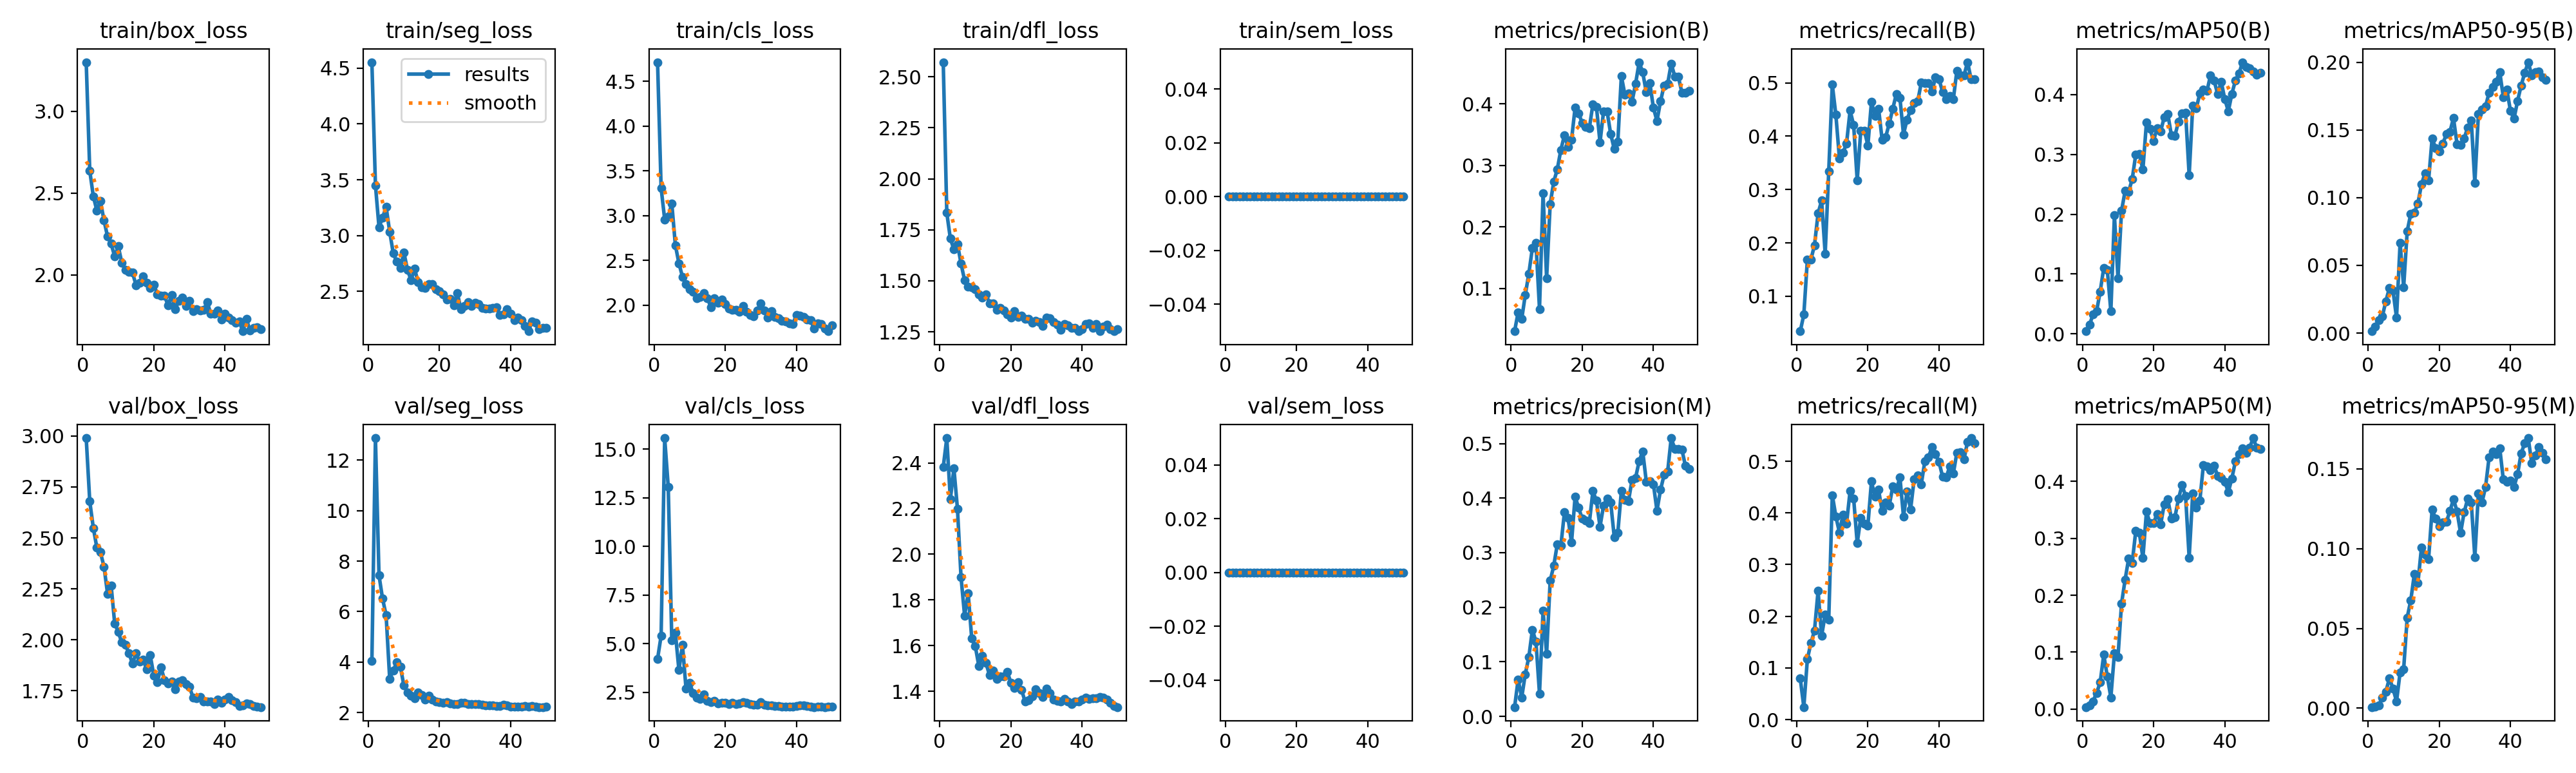
\includegraphics[width=0.86\textwidth]{yolo_finetune_results.png}
\caption{Curvas de entrenamiento y validación del modelo fine-tune.}
\label{fig:yolofinetune}
\end{figure}

\begin{figure}[H]
\centering
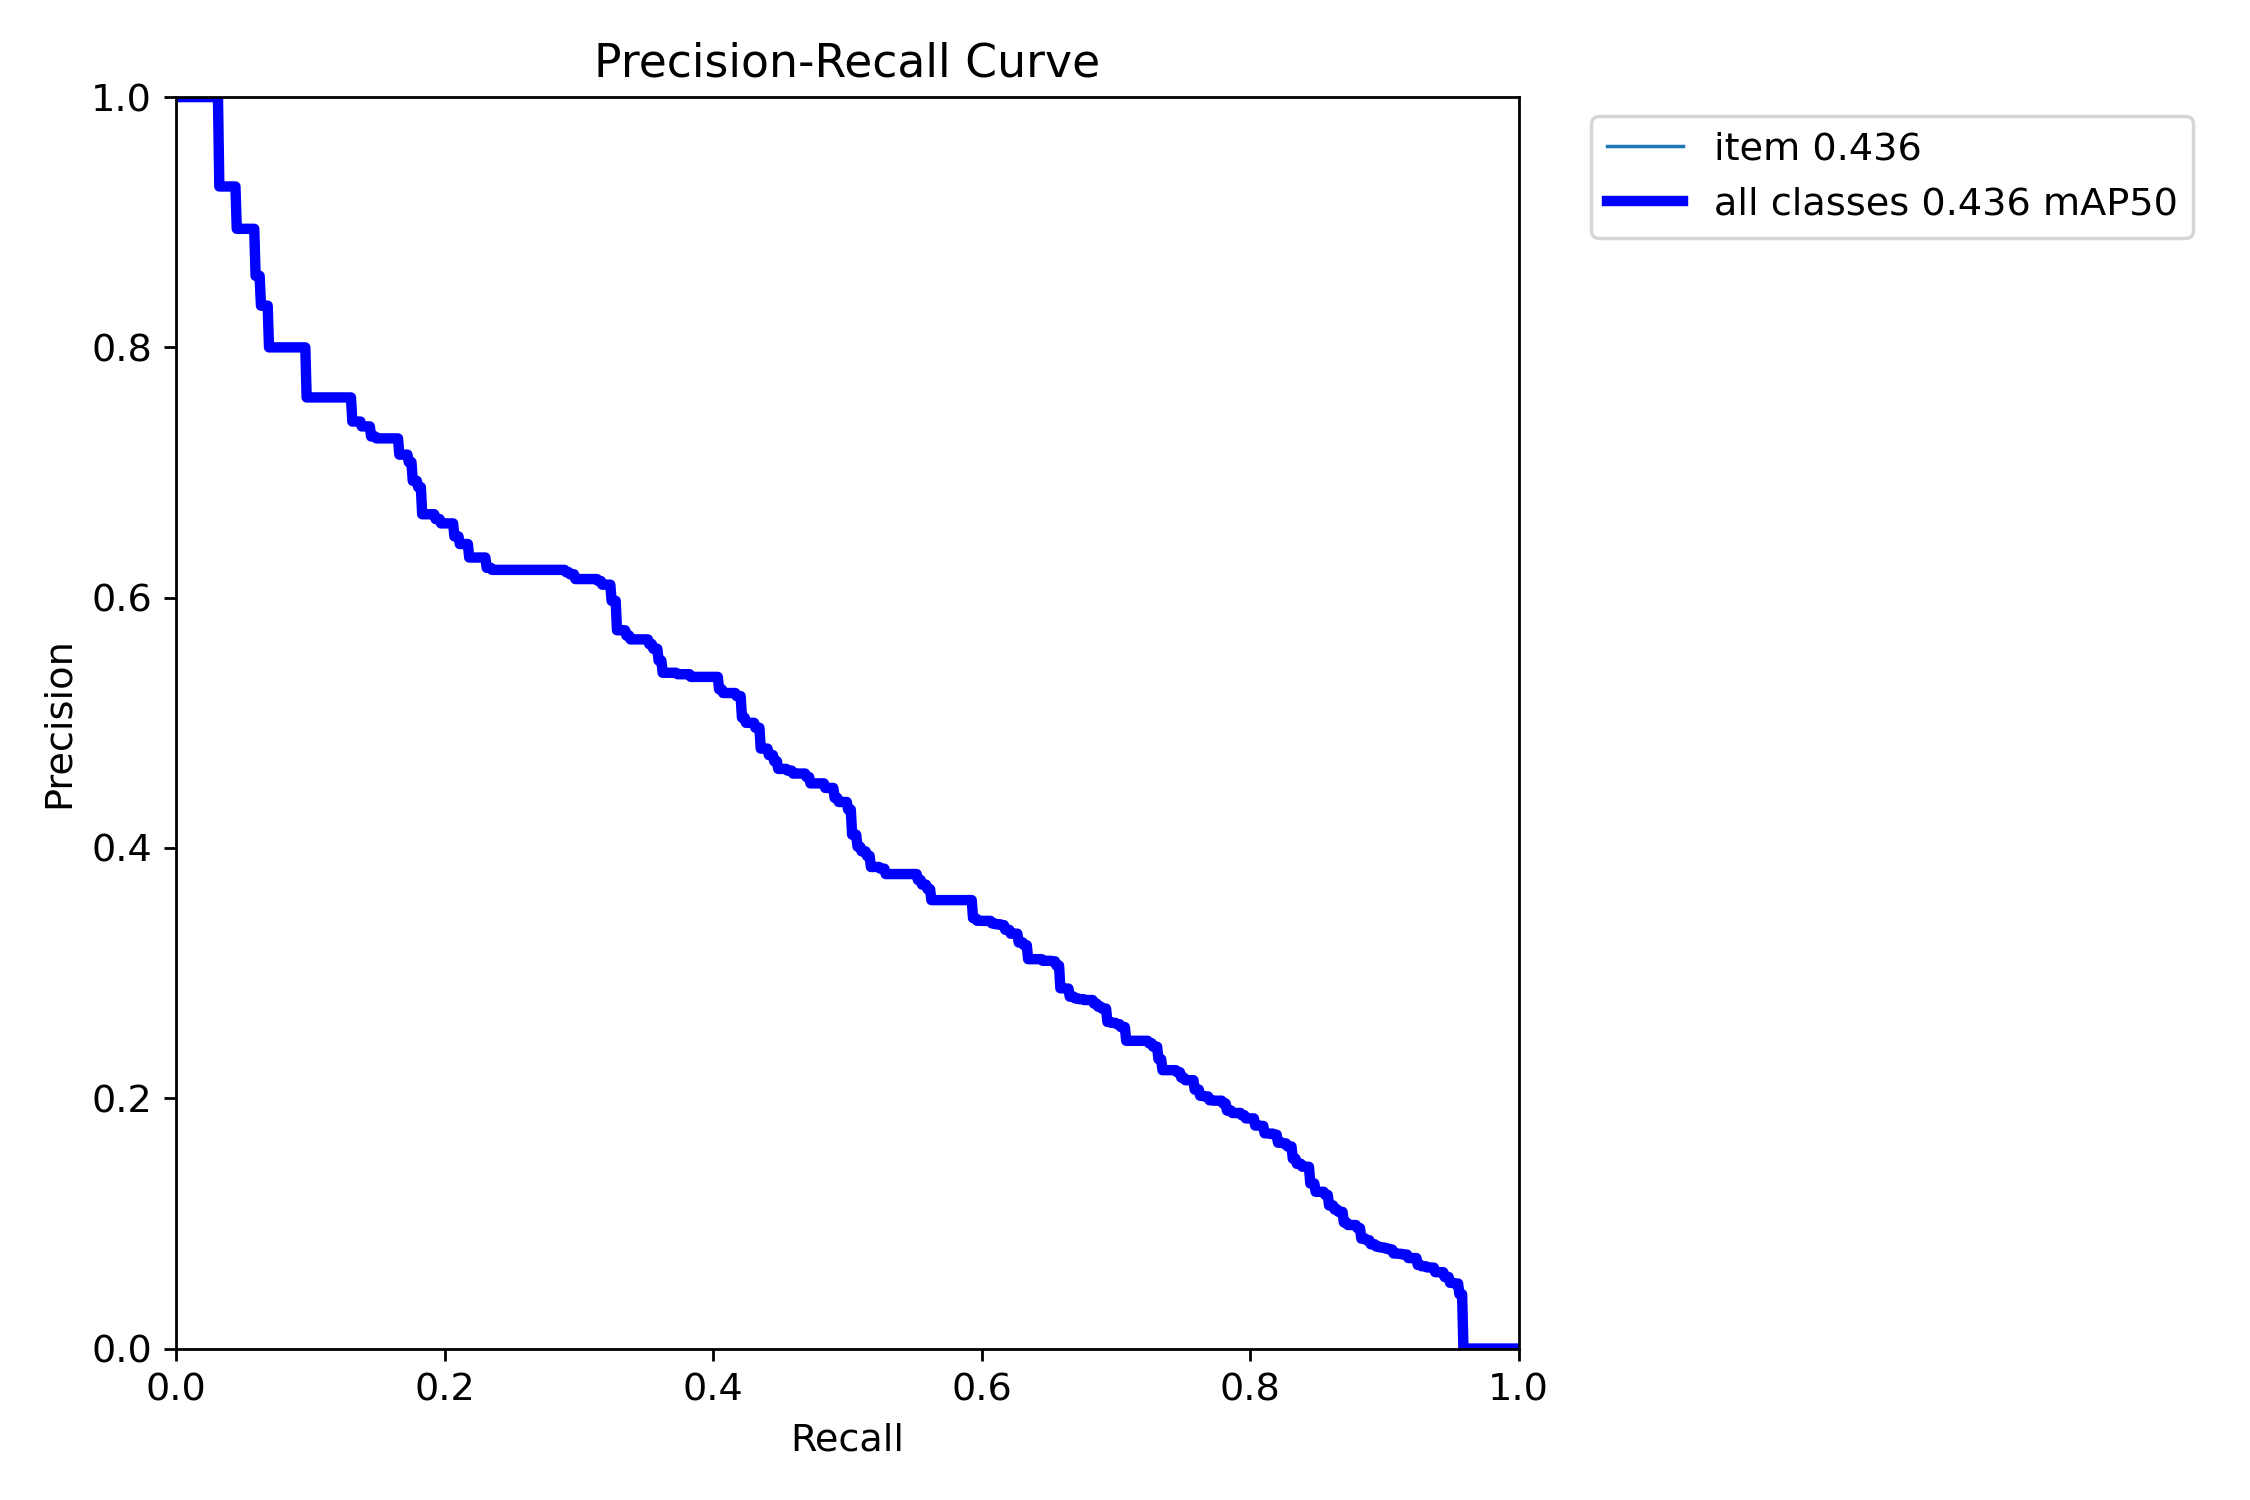
\includegraphics[width=0.78\textwidth]{yolo_transfer_mask_pr.png}
\caption{Curva precisión-recall de máscaras en el modelo con transferencia.}
\label{fig:transferpr}
\end{figure}

\begin{figure}[H]
\centering
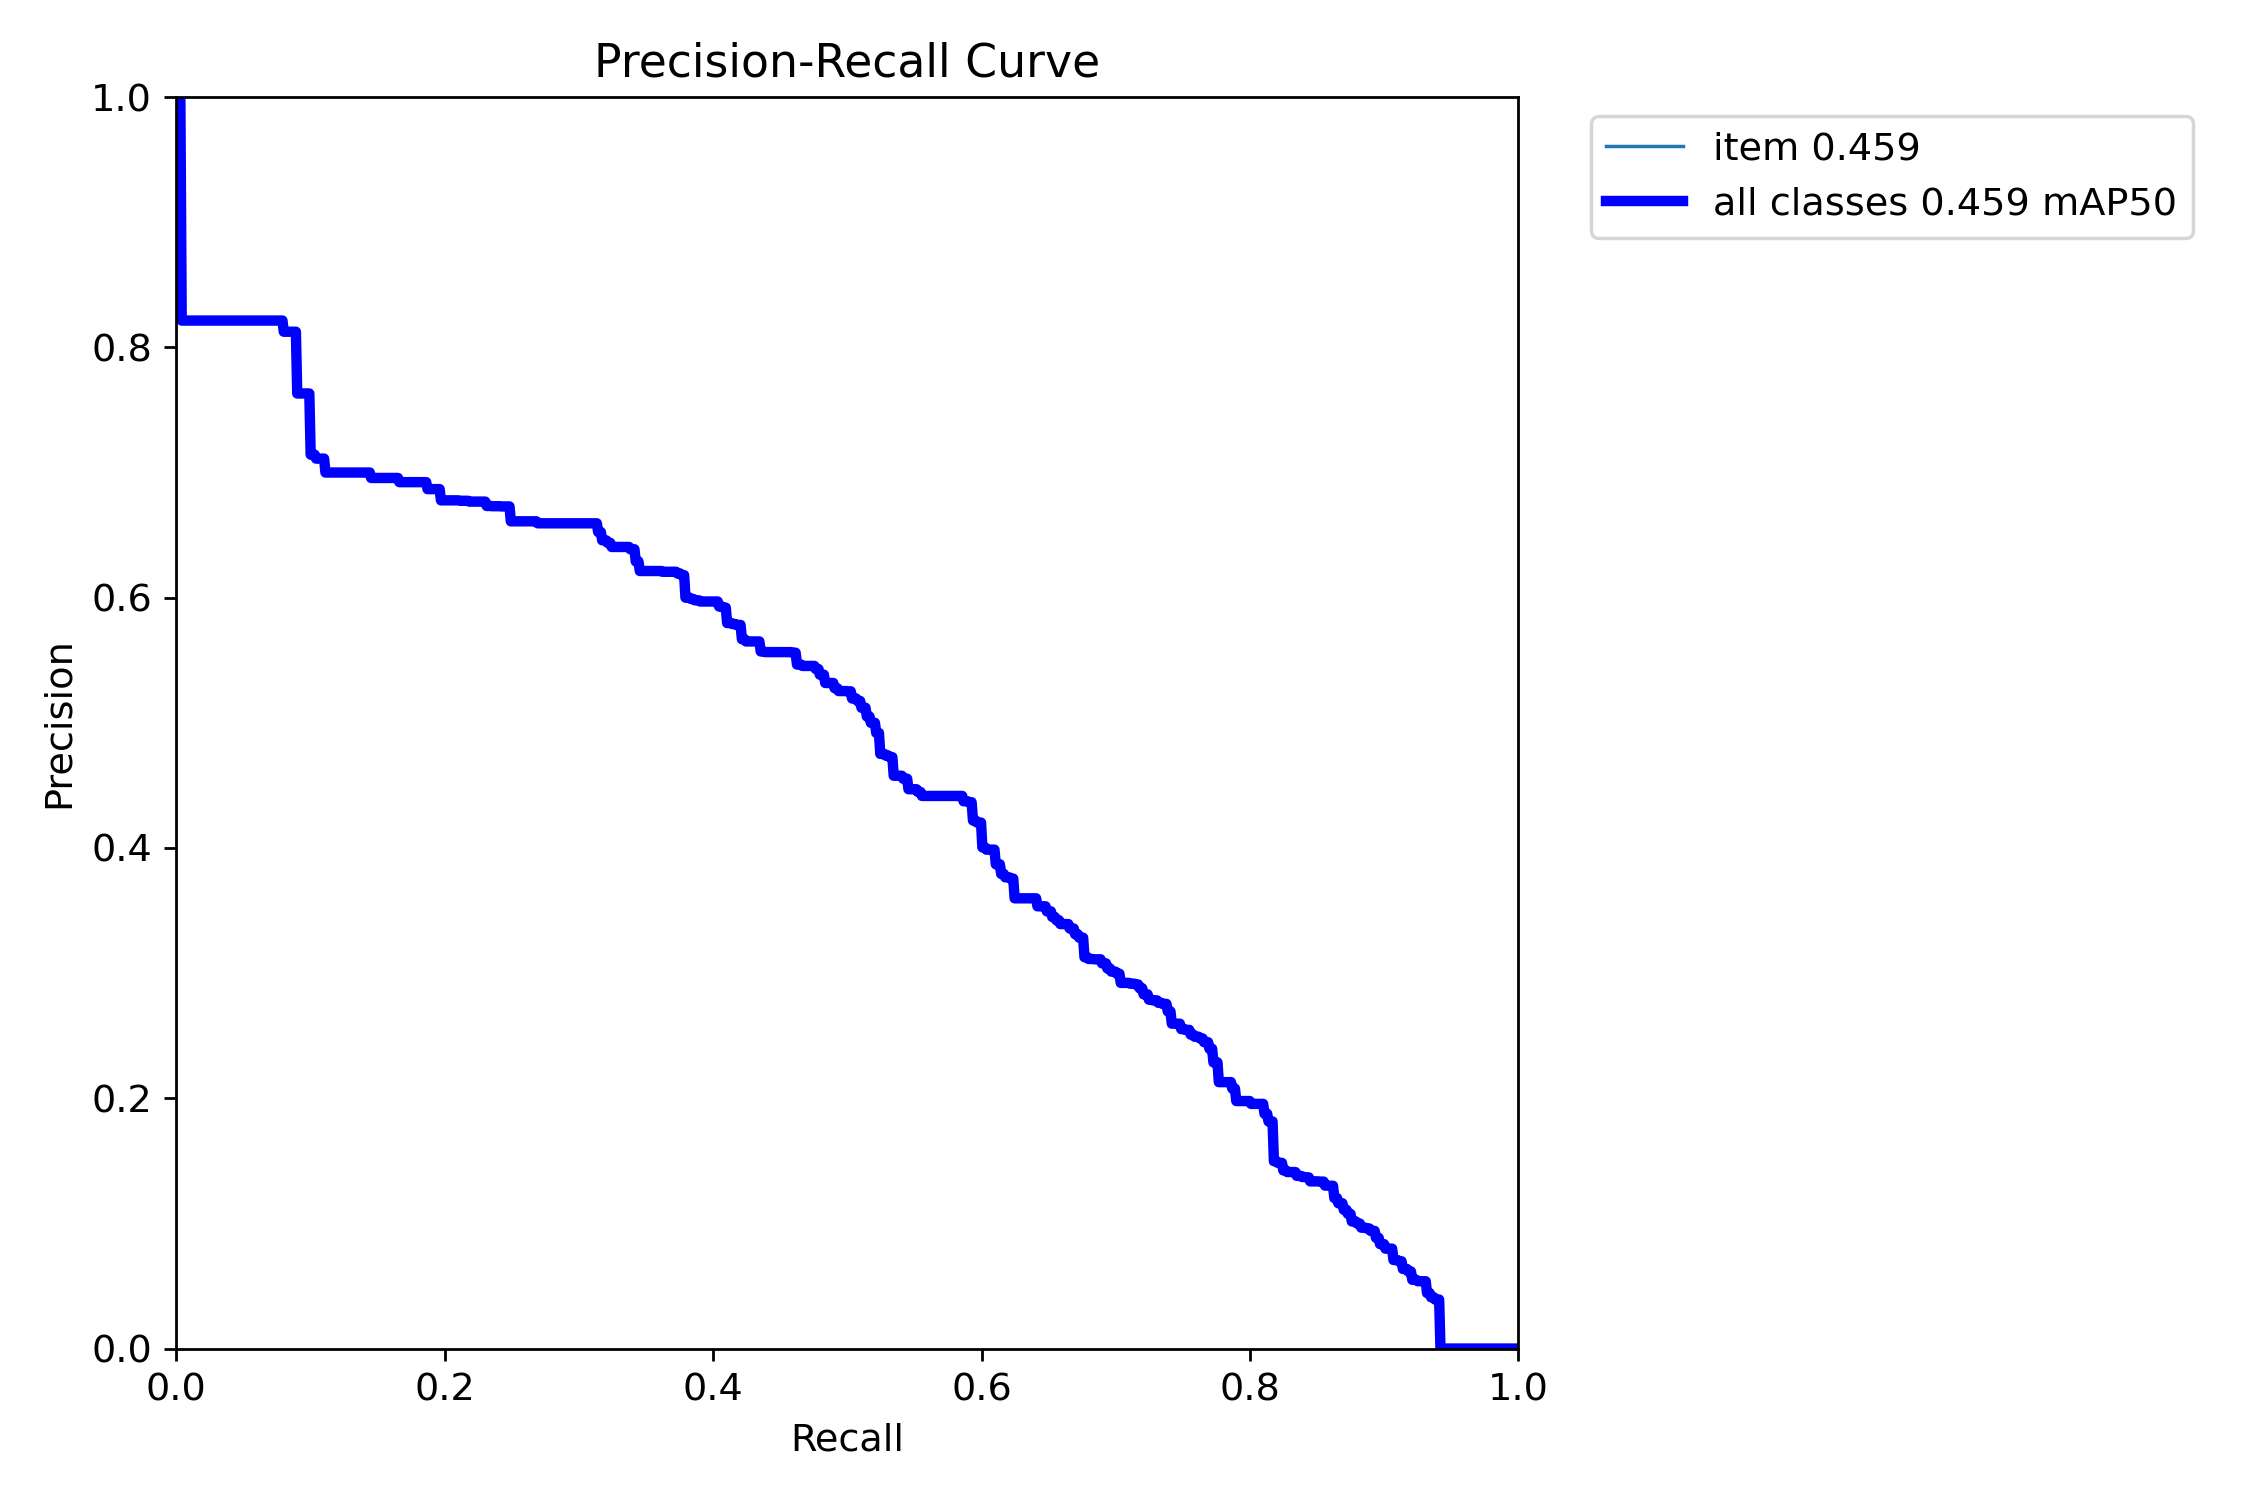
\includegraphics[width=0.78\textwidth]{yolo_finetune_mask_pr.png}
\caption{Curva precisión-recall de máscaras en el modelo fine-tune.}
\label{fig:finetunepr}
\end{figure}

Las predicciones visuales permiten revisar errores que las curvas agregadas no muestran. Se observan fragmentos perdidos, contornos imperfectos y detecciones que no coinciden completamente con las máscaras reales.

\begin{figure}[H]
\centering
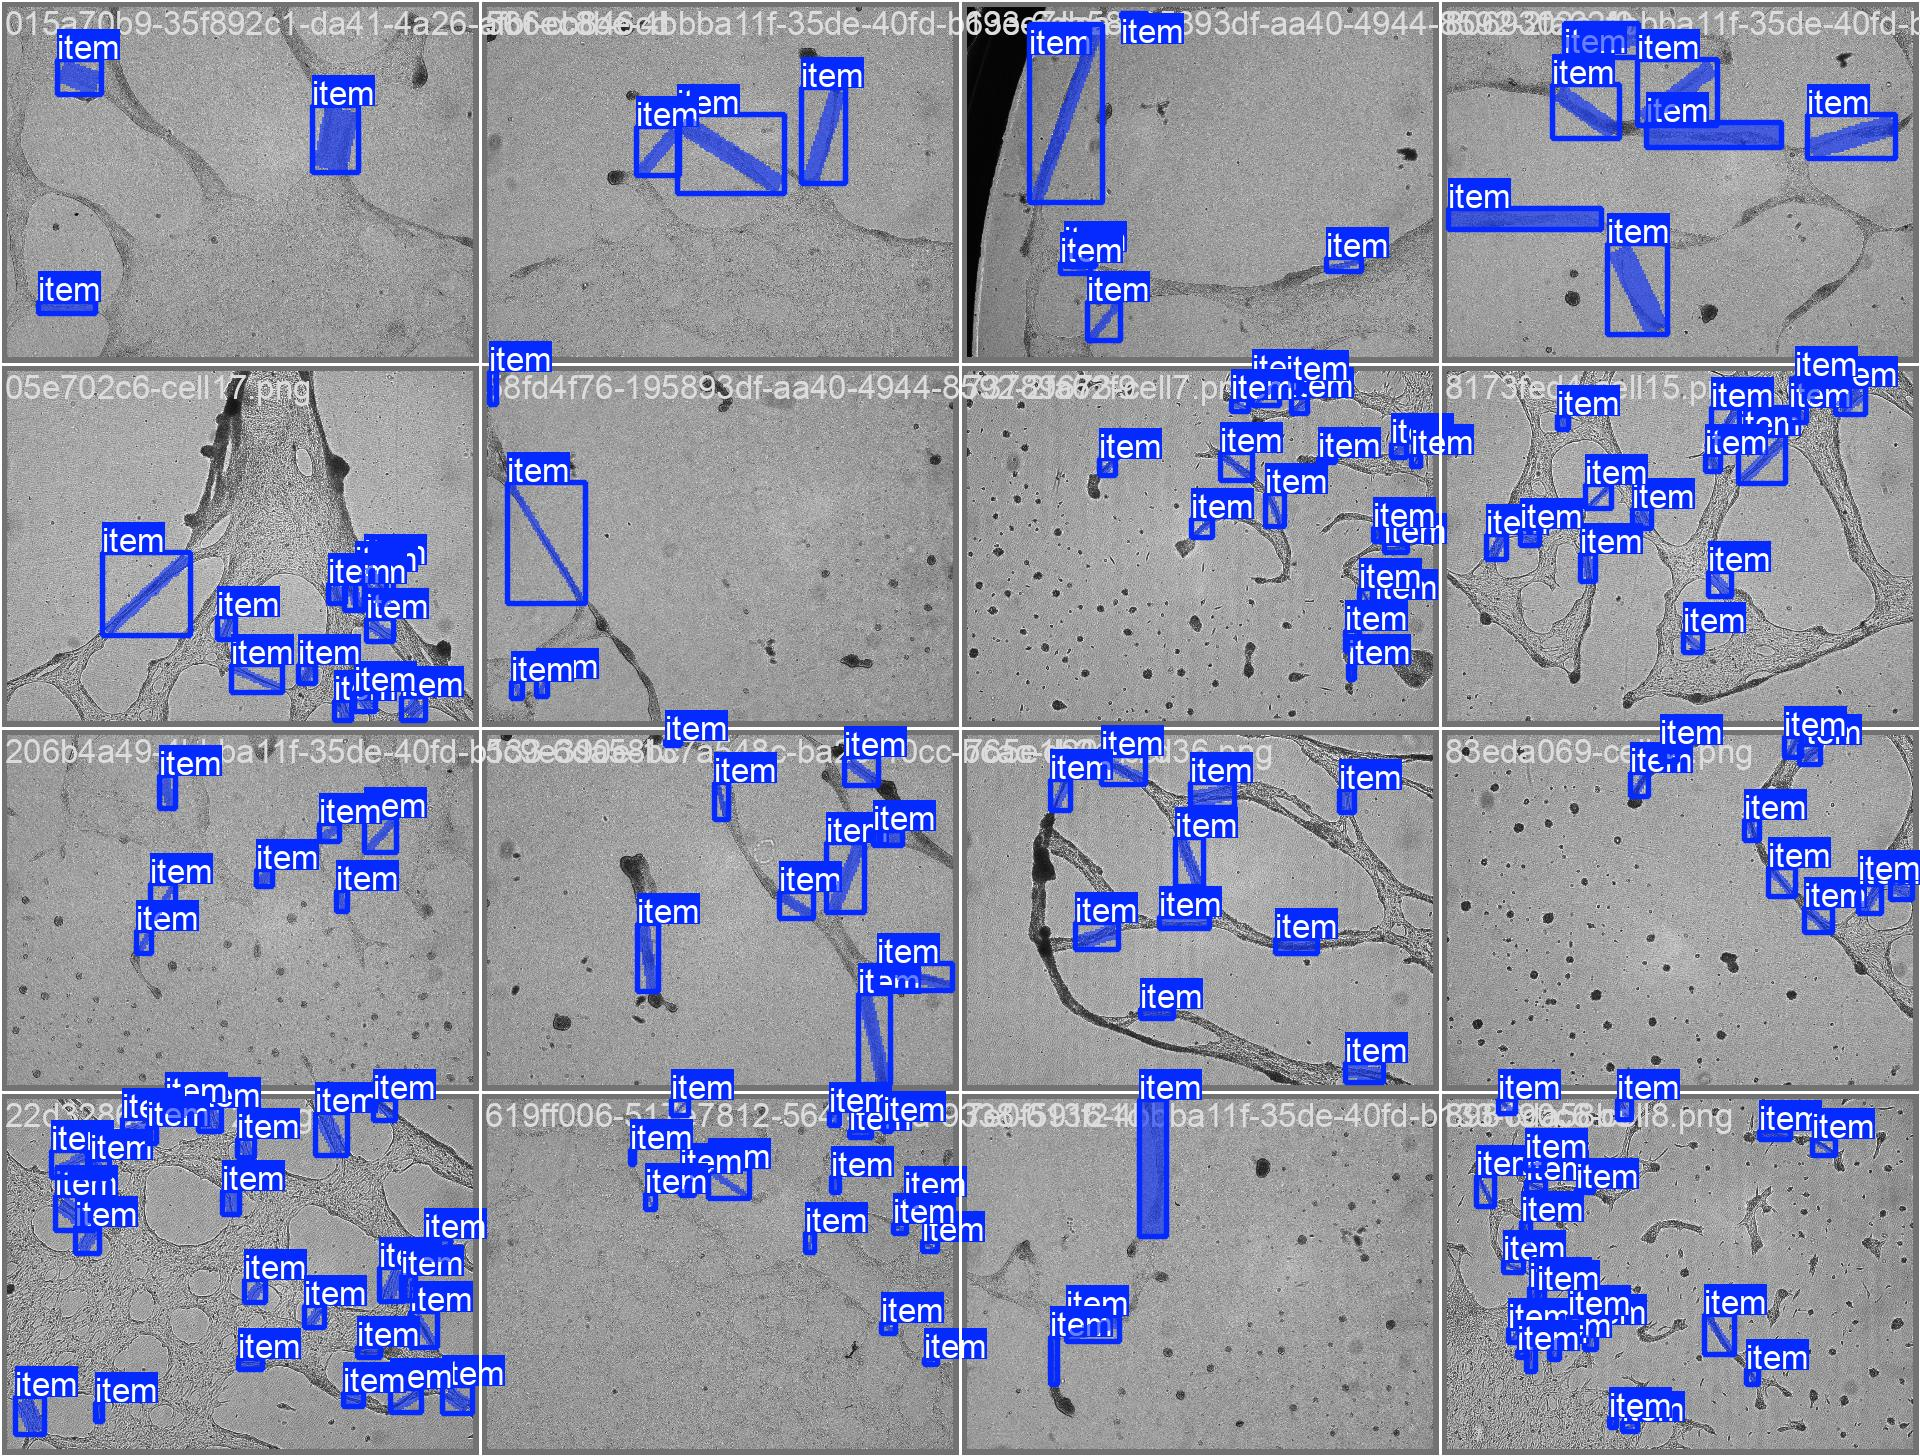
\includegraphics[width=0.82\textwidth]{yolo_transfer_val_labels.jpg}
\caption{Etiquetas de referencia en un lote de validación del modelo con transferencia.}
\label{fig:transferlabels}
\end{figure}

\begin{figure}[H]
\centering
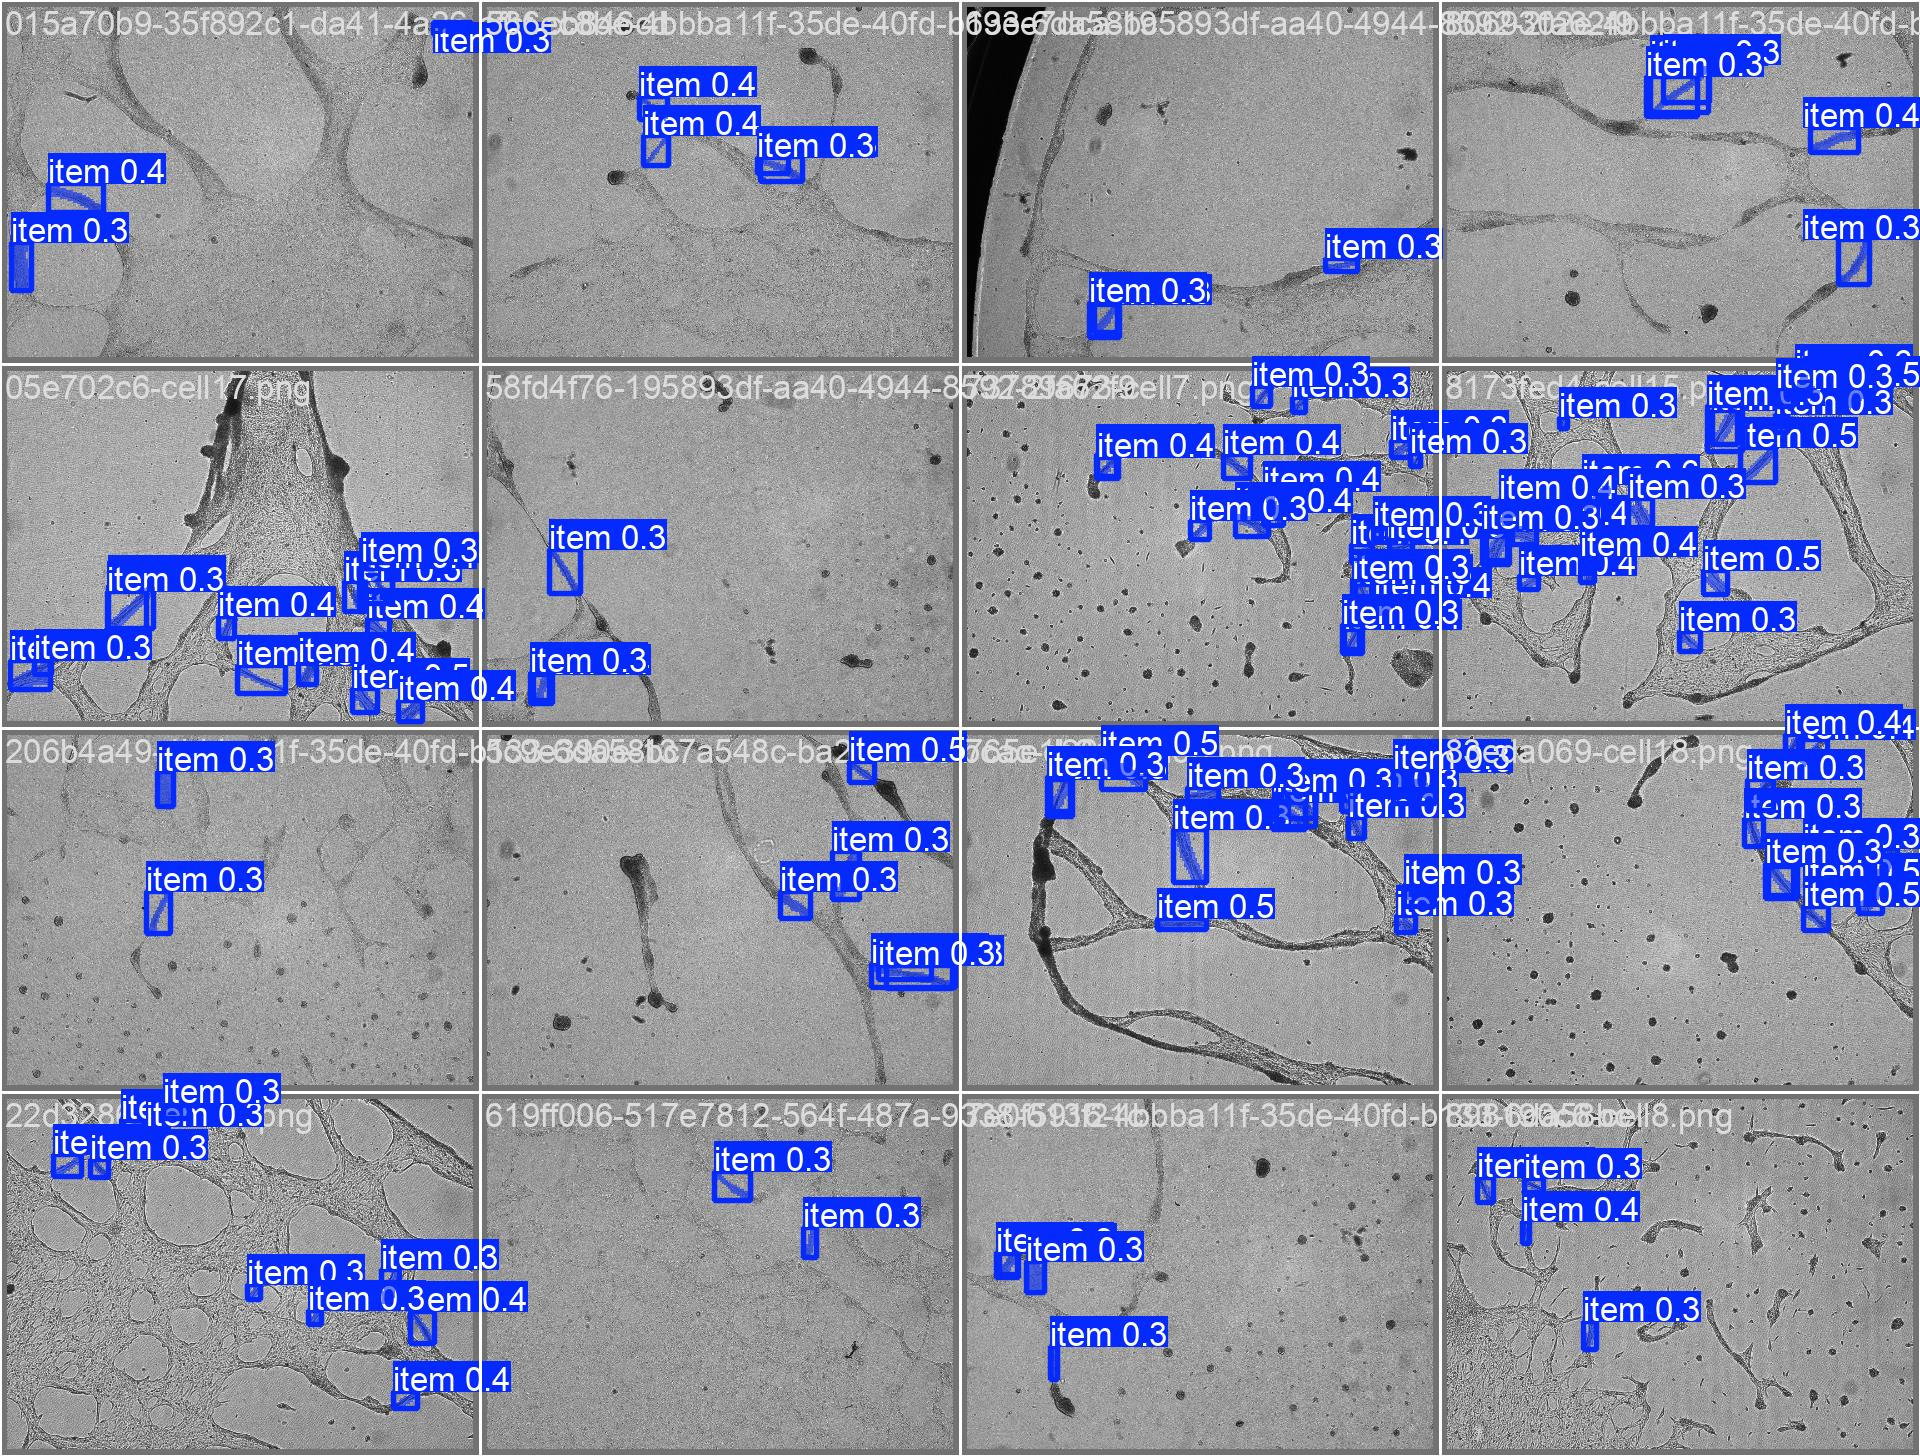
\includegraphics[width=0.82\textwidth]{yolo_transfer_val_pred.jpg}
\caption{Predicciones del modelo con transferencia sobre el lote de validación.}
\label{fig:transferpred}
\end{figure}

\begin{figure}[H]
\centering
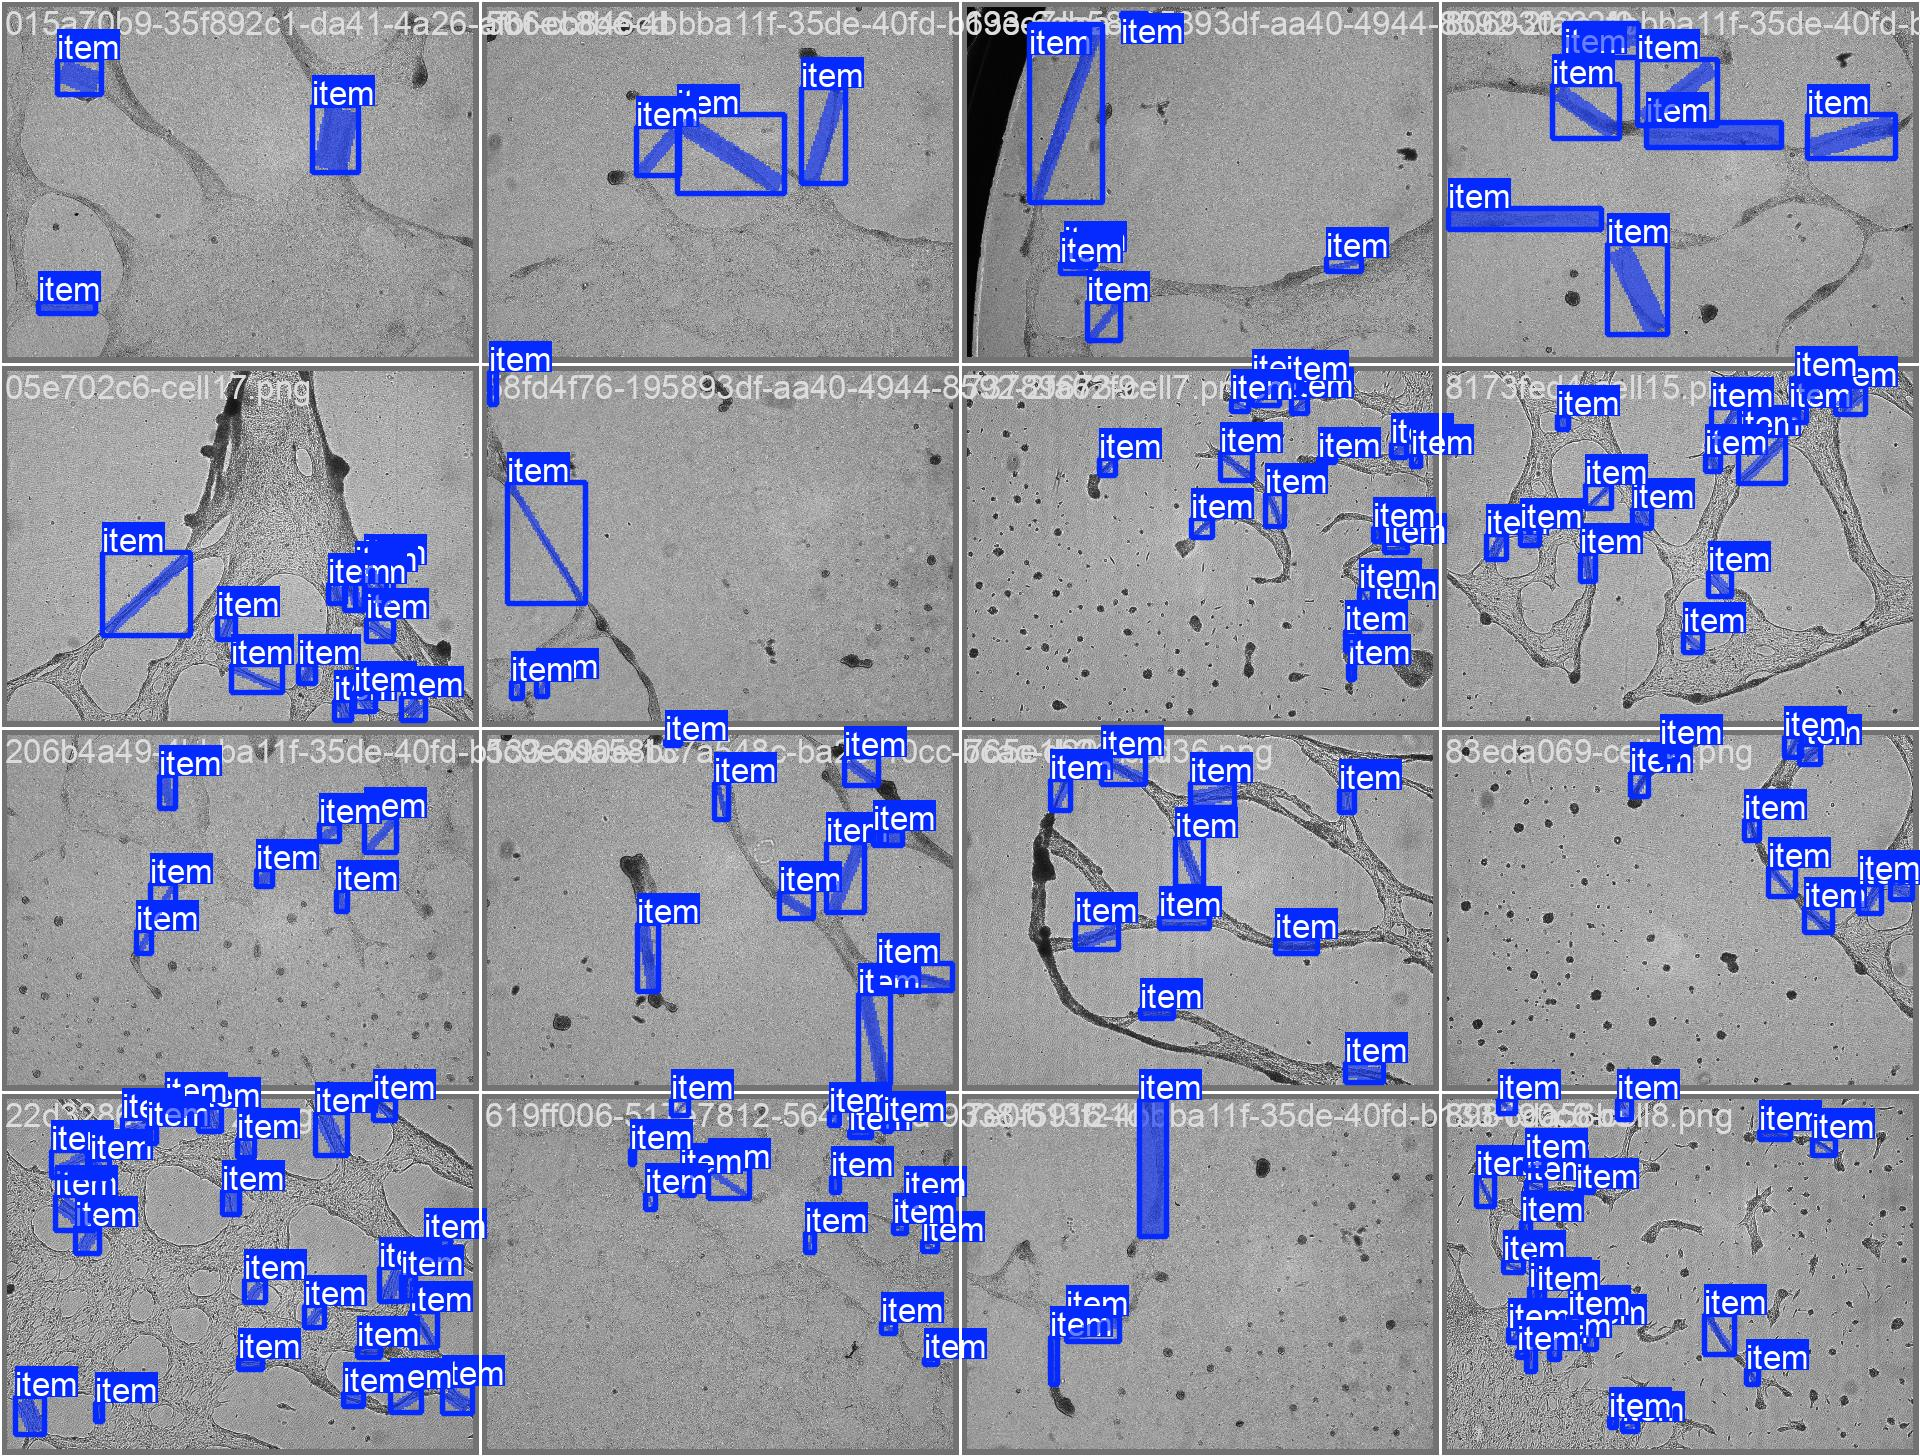
\includegraphics[width=0.82\textwidth]{yolo_finetune_val_labels.jpg}
\caption{Etiquetas de referencia en un lote de validación del modelo fine-tune.}
\label{fig:finetunelabels}
\end{figure}

\begin{figure}[H]
\centering
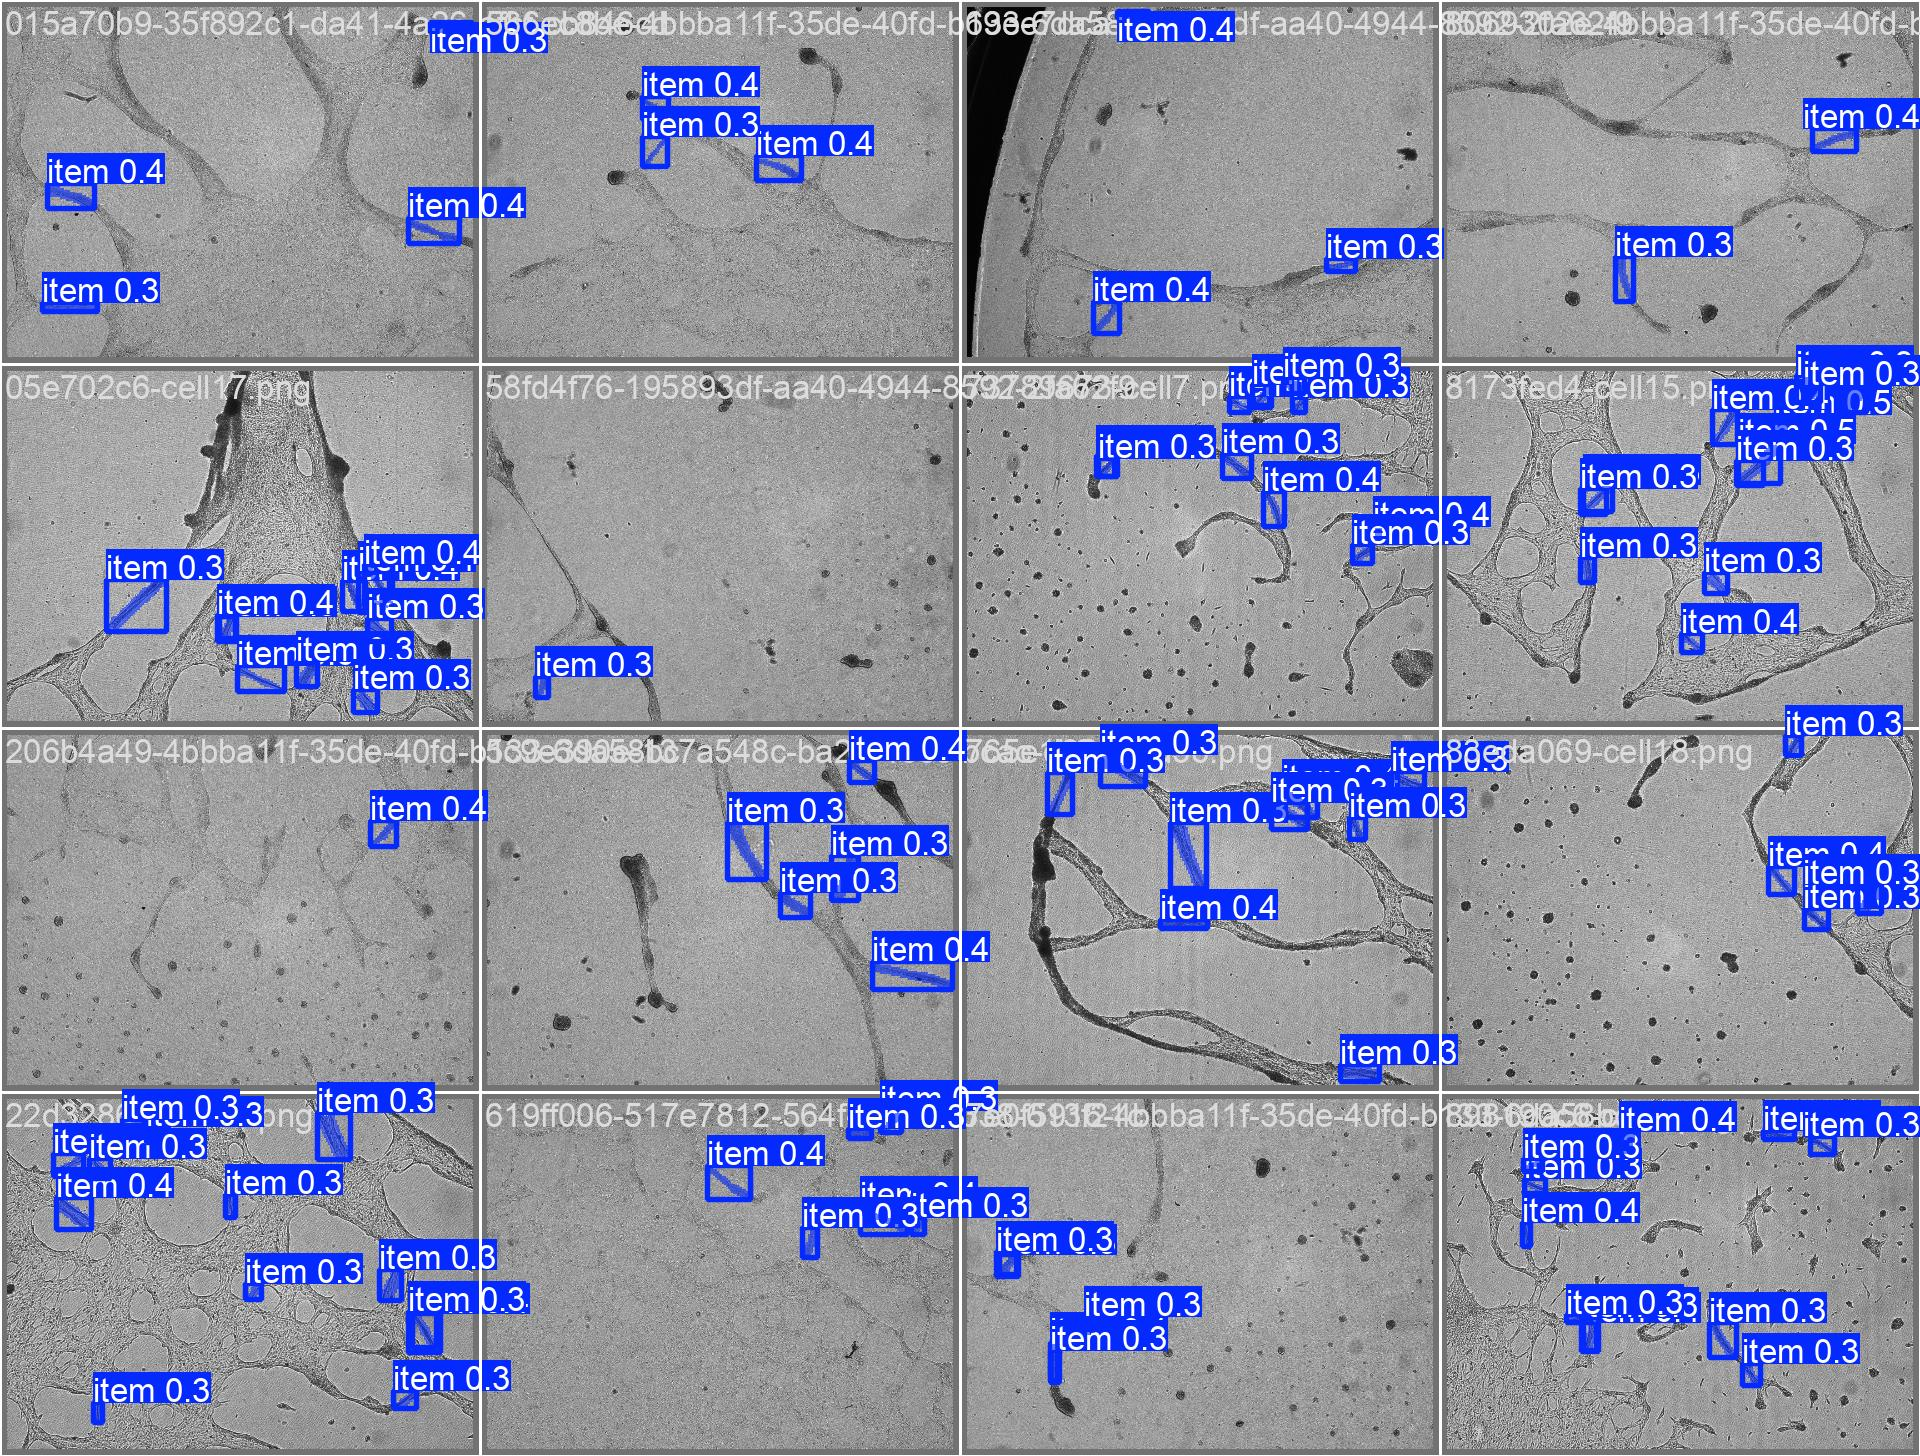
\includegraphics[width=0.82\textwidth]{yolo_finetune_val_pred.jpg}
\caption{Predicciones del modelo fine-tune sobre el lote de validación.}
\label{fig:finetunepred}
\end{figure}

\section{Discusión}

El componente más importante del proceso fue controlar el agrupamiento de réplicas. Sin esta restricción, la validación sobreestima el rendimiento por la cercanía visual entre imágenes relacionadas.

El desbalance limita tanto las líneas base como los modelos de segmentación. El fondo representa casi el 98.3\% del conjunto original. Las métricas globales pueden quedar dominadas por el fondo, por lo que IoU y Dice del miotubo ofrecen una lectura más relevante del problema.

Entre las líneas base, el clasificador HGB obtiene mejores resultados generales. Sin embargo, su recall a alta precisión es casi nulo. Entre los modelos YOLO, fine-tune supera a transferencia en los máximos mAP50 y mAP50-95. Esa mejora no elimina la necesidad de una evaluación independiente en prueba.

\section{Conclusiones}

La calidad de los datos es suficiente para realizar experimentos, pero presenta casos de anotación incompleta y variación morfológica. Las máscaras vacías requieren revisión antes de tratarlas como negativos reales.

La partición agrupada eliminó el solapamiento aparente por réplicas. La estrategia debe conservarse en futuras experimentaciones para evitar una medición optimista.

El clasificador de píxeles supera a la línea clásica en PR-AUC, ROC-AUC e IoU de miotubo. Fine-tune supera a la variante de transferencia en los indicadores YOLO de máscaras.

Los mejores resultados existentes siguen siendo insuficientes para un uso clínico o automático. Antes de selección final conviene evaluar el conjunto de prueba, revisar imágenes con máscaras inconsistentes y ampliar el análisis por tipo de apariencia y por imagen.

\section{Reproducibilidad}

La partición usa semilla 42 y queda registrada en \texttt{data/processed/splits}. Los parámetros de las dos ejecuciones YOLO están guardados en \texttt{args.yaml}. Las tablas y figuras de este informe están disponibles en \texttt{reports} y \texttt{reports/figures}.

\section{Comparación clásica frente a deep learning}

El clasificador de píxeles y YOLO usan unidades de evaluación distintas. El clasificador informa métricas píxel a píxel en validación, mientras YOLO informa detección de máscaras, precisión y recall de instancia, junto con mAP. Las cifras no son intercambiables sin una evaluación conjunta. Incluso así, permiten una comparación inicial cuando se añaden puntuaciones compatibles.

\begin{table}[H]
\centering
\small
\caption{Comparación inicial de enfoques sobre validación.}
\begin{tabular}{lrrrr}
\toprule
Modelo & Dice píxel & IoU píxel & Precisión & Recall\\
\midrule
HGB clásico & 0.2832 & 0.1650 & 0.3084 & 0.2618\\
YOLO transferencia & No disponible & No disponible & 0.4574 & 0.4690\\
YOLO fine-tune & No disponible & No disponible & 0.4891 & 0.5379\\
\bottomrule
\end{tabular}
\end{table}

El HGB obtiene 0.2832 de Dice y 0.1650 de IoU a nivel píxel. YOLO no registra esos resultados con la misma máscara binaria en los informes disponibles. Su precisión y recall de máscaras son mayores que los del clasificador, especialmente en fine-tune. Fine-tune alcanza además 0.4763 de mAP50 y 0.1692 de mAP50-95, frente a 0.4364 y 0.1596 en transferencia.

La comparación indica que el enfoque clásico es una línea base útil y económica. Produce métricas por píxel claras, pero su recall permanece bajo y no aprovecha patrones espaciales ni contextuales complejos. YOLO ofrece mejores precisión y recall de máscara y su fine-tune supera a la variante con capas congeladas.

Se recomienda continuar con deep learning como dirección principal. Esta decisión debe mantenerse provisional hasta calcular para YOLO el Dice píxel, el IoU píxel y otras métricas por imagen con el mismo conjunto de validación y umbrales del HGB. También conviene evaluar el conjunto de prueba antes de descartar el enfoque clásico. HGB puede conservarse como referencia y como posible modelo de apoyo o validación rápida.

\end{document}
